\documentclass[final,11p]{CSP}
\usepackage{amssymb}
\usepackage{changepage}
\usepackage{float}
\usepackage{hyperref}
\usepackage{url}
\usepackage{afterpage}
\usepackage{natbib}
\usepackage{setspace}
\usepackage{fancyhdr}
\pagestyle{fancy}
\fancyhf{}

\def\Student{Ashish Sehrawat}
\def\Director{Dr. Jos\'{e} Feliciano Ben\'{i}tez Rubio}
\def\Title{MONOGRAPH}
\def\Prog{Doctorado en Ciencias (F\'{i}sica) }
\def\Dept{Departamento de Investigac\'{i}on en Fis\'{i}ca}
\def\Division{Division de Ciencias Exactas y Naturales}
\def\Universidad{Universidad de Sonora}

\def\ProjectTitle{Luminosity measurement with the Pixel detector at the CMS experiment of the Large Hadron Collider }
\def\ResearchLine{Astrof\'{i}sica, Cosmolog\'{i}a y F\'{i}sica de Part\'{i}culas}


\newcommand{\SubItem}[1]{
    {\setlength\itemindent{15pt} \item[-] #1}
}


%%header and footer
\lhead{\Student / \Prog }
\rhead{\Title}
\lfoot{\Dept}
\rfoot{Page \thepage}
\setlength{\headsep}{0.2in}
\renewcommand{\footrulewidth}{0.4pt}% default is 0pt


\begin{document}

%%%%Cover page
\begin{titlepage}
  \centering
  \hspace{0pt}
  \vfill
        {\scshape\Large \Title \par}

	\vspace{2cm}
        %\begin{adjustwidth}{2cm}{2cm}{
        %    TITLE:\par
            {\large \bf \ProjectTitle \par}
        %  }
        %\end{adjustwidth}

%	\vspace{0.5cm}
%        \begin{adjustwidth}{2cm}{2cm}{
%            RESEARCH LINE: \par
%            \ResearchLine \par}
%        \end{adjustwidth}

        
        \vspace{4cm}
        %{\underline{\hspace{8cm}}\par}
	{\scshape\large \Student \par}
        {PhD. Student\par}

        \vspace{1cm}
        %{\underline{\hspace{8cm}}\par}
	{\scshape \Director \par}
        {Thesis Director\par}

        \vspace{1cm}
        {\bf \Prog \par}
        {\Dept \par}
        {\Division \par}
        {\scshape \Universidad \par}

        \vspace{4cm}
	{\today}

\hspace{0pt}
\vfill

\end{titlepage}
%%%%% white page for print out
\shipout\null

%%%% Title and Abstract Page
\newpage
\hspace{11pt}
%\vfill

\begin{adjustwidth}{1cm}{1cm}

  \begin{center}
    {\Large \ProjectTitle \par}
    \vspace{0.5cm}

    {\Student \par}
    {\Universidad \par}  
    \vspace{1cm}
    
    {\itshape\textbf{Abstract}\par}
     \vspace{0.7 cm}
        
    \end{center}  

 
  \onehalfspacing The Pixel Cluster Counting (PCC) luminosity measurement method is an offline technique for the calculation of luminosity for any LHC run period based on counting the number of pixel clusters in the CMS pixel detector (innermost part of the CMS tracker) using minimum bias events. We investigate stability of PCC luminosity using 2018 CMS data for various subdetectors in the upgraded Phase I pixel detector. For Run 2 data, we aim to achieve a 1\% uncertainty on the final luminosity measurement. Also, we develop the algorithms and optimization for the Phase II High Luminosity LHC (HL-LHC) luminosity measurement using the Tracker Endcap Pixel Detector (TEPX) for which excellent statistical and linearity performance is expected.


    
\end{adjustwidth}

\hspace{2pt}
%\vfill
\vspace{1 cm}

%%%%%%%%%%%%%%%%%%%
\clearpage
\shipout\null


%%%%%% Begin the body
\newpage
%\onehalfspacing
\tableofcontents

\clearpage
\newpage
In Run III and HL-LHC phases, the LHC is expected to run at peak instantenous luminosities of about 2\ \instlumiunit\ and 5-7\ \instlumiunit, respectively \cite{hllhc}.
For the HL-LHC the proton bunch intensities will increase and will cause the pileup to reach peak values of 140-200, by comparison the Run II average pileup was about 34 with peak values around 50. 
During 2018, runs with special trigger configuration were recorded with pileup up to 100, these runs allow for studies of the effects of high pileup on the relative linearity between luminometers.
The luminosity measurement based on Pixel Cluster Counting (PCC) \cite{CMS-PAS-LUM-12-001,CMS-PAS-LUM-13-001,PCC2016_publicplots} method is expected to have a good linearity to high pileup due to its fine granularity.  


\section{The Large Hadron Collider}
\label{sec:lhc}
(describe the accelerator complex, proton bunches, c.m. energy, all experiments, run periods, inst. and integrated lumi, Run 3 and HL-LHC plans) \\

\onehalfspacing CERN accelerator complex is a progression of machines namely Linac 2, Proton Synchrotron Booster (PSB), Proton Synchrotron (PS), Super Proton Synchrotron (SPS) and Large Hadron Collider (LHC) as shown in Fig. 1 that accelerate particles mainly protons to increasingly higher energies of 50 MeV, 1.4 GeV, 25 GeV, 450 GeV and 14 TeV respectively. Each machine is used to increase the energy of particle before the beam is injected into to the next machine. Linear accelerator (Linac2) is the starting point for protons used in various experiments at CERN. After proton energy reaches 50 MeV, protons enter PSB which further increases its energy before they are injected into PS which takes up its energy to 25 GeV. After reaching 25 GeV, protons enter SPS which further increases its energy to 450 GeV. The protons are finally transferred to two beam pipes of LHC kept at very high vacuum.  \\ 

The Large Hadron Collider (LHC) is the most powerful particle accelerator in the world primarily build to collide protons and heavy ions at 7, 8, 13 and 14 TeV during different LHC run period. The LHC consists of a 27 kilometre ring of superconducting magnets producing strong magnetic field which is used to guide particle beams along the LHC ring. Proton beam made up of bunches travelling in opposite directions kept in two ultrahigh vacuum tubes are accelerated close to the speed of light using time dependent electric field produced by radiofrequency cavities before they collide at four interaction points along the LHC ring where ATLAS, ALICE, CMS and LHCb detectors are placed. \\

The first proton beam was successfully maneuvered around the LHC ring in September 2008 that marked the beginning of Run 1 with proton beams colliding at 7-8 TeV center-of-mass energy and this run period ended in 2013. Run 2 started in 2015 with protons colliding at 13 TeV center-of-mass energy and continued till October 2018. Run 3 is expected to begin at the start of March 2022 and High Luminosity (HL)-LHC phase is expected to begin in mid-2027. Proton Synchroton (PS) is responsible for providing proton bunches spaced 7 metres (25 ns) apart with each bunch containing more than 100 billion protons. The maximum number of bunches reached with the beam preparation method used during Run 2 is 2556. The number of protons in the colliding bunches, time of separation between the bunches and effective area of the bunch which depend on the rms transverse bunch size along horizontal and vertical directions is one of the ways to calculate instantaneous luminosity (L_{inst}). \\

Luminosity is a key performance parameter of an accelerator as it is a measure of number of collisions. Luminosity can be categorized into two types: instantaneous and integrated luminosity. Instantaneous luminosity is defined as the number of collisions occuring per second in per centimeter square area while integrated luminosity is obtained by integrating instantaneous luminosity over a time interval. Both are very important variables as they are used to obtain the number of collision events. During Run 1, peak value of LHC instantaneous luminosity was $0.77 \times 10^{34} \: cm^{-2} s^{-1} $ with $30 \: fb^{-1}$ integrated luminosity. During Run 2, LHC instantaneous luminosity reached a peak value of $1.58 \times 10^{34}  \: cm^{-2} s^{-1}$ with $150 \: fb^{-1}$ integrated luminosity as shown in Fig. 2. At the end of Run 3, we expect to achieve an integrated luminosity  of $300 \:fb^{-1}$ while Phase 2 HL-LHC is expected to collect $3000 \:fb^{-1}$ of data as shown in Fig. 3 thereby increasing luminosity by a factor of 10 beyond the LHC's design value. \\


\begin{figure}[H]
  \centering
  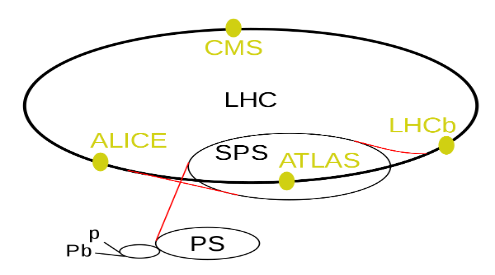
\includegraphics[width=0.8\columnwidth]{./LHCcomplex.png}
  \caption{\onehalfspacing Diagram of the LHC accelerator complex located in Geneva, Switzerland. Four interaction points are shown for the ALICE, ATLAS, LHCb and CMS experiments.}
  \label{fig:LHC}
\end{figure}


\begin{figure}[H]
  \centering
  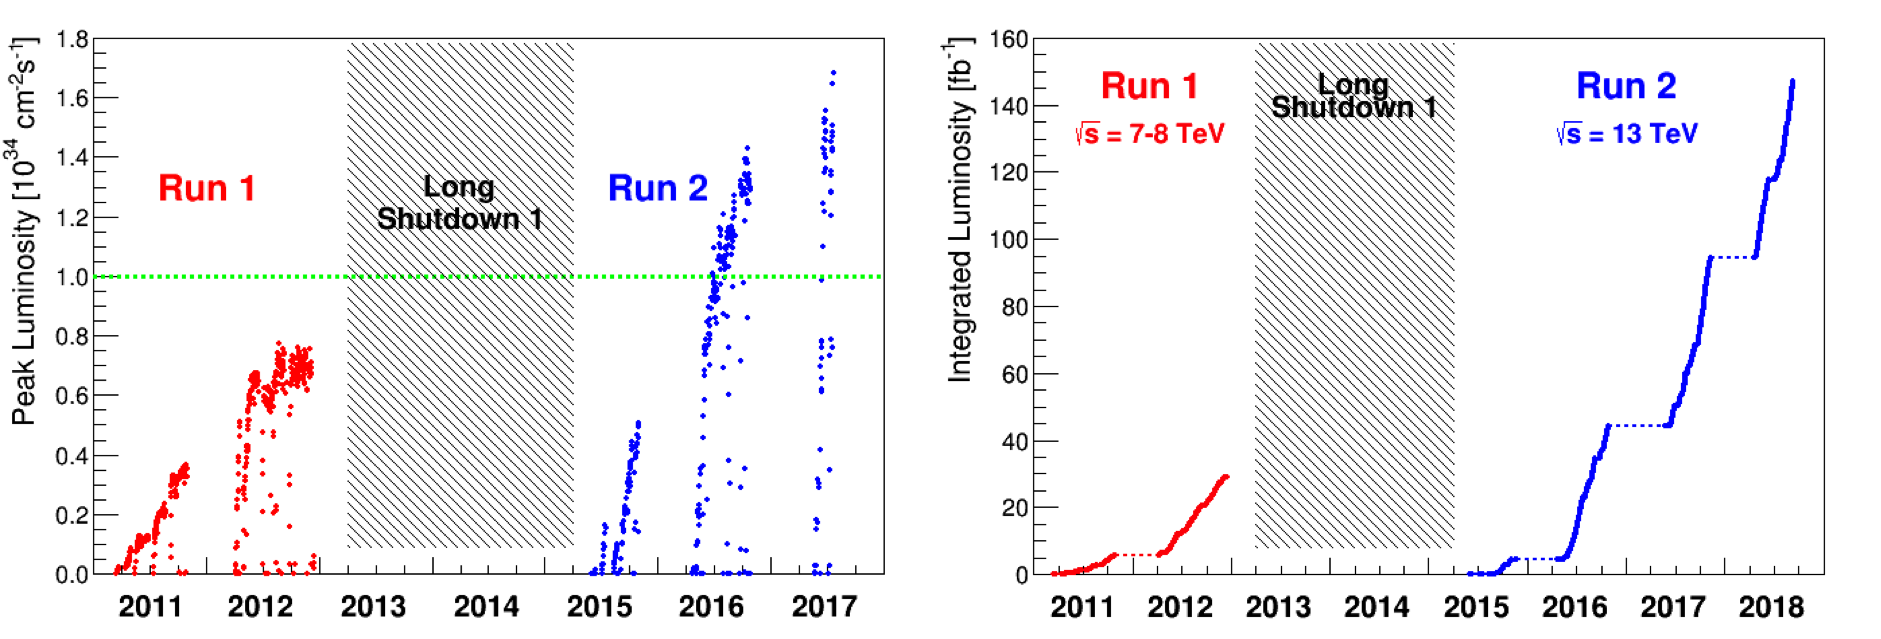
\includegraphics[width=1 \columnwidth]{./run1-2_lumi.png}
  \caption{\onehalfspacing Left: Instantaneous luminosities for Run 1 and Run 2 period. Right: Integrated luminosities for Run 1 and Run 2 period.}
  \label{fig:LHClumi}
\end{figure}


\begin{figure}[H]
  \centering
  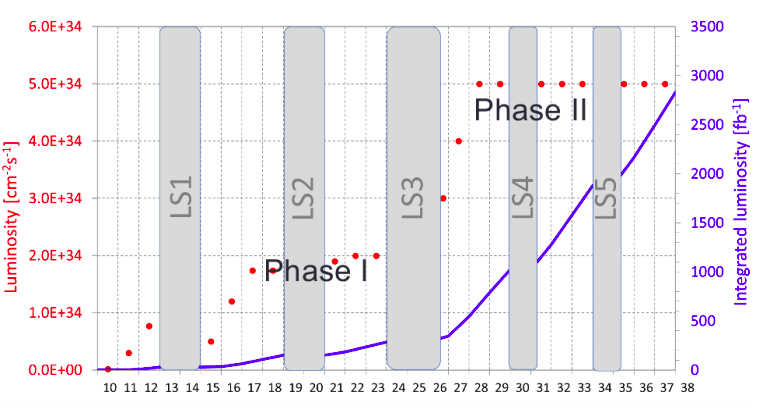
\includegraphics[width=0.7 \columnwidth]{./lumi_projection.png}
  \caption{ \onehalfspacing Projected performance of the LHC until 2038, which shows the preliminary dates for prolonged stops (LS1, LS2, LS3, LS4, LS5) of the LHC and luminosities. Red points show instantaneous luminosity $(L_{inst})$ while the blue line shows integrated luminosity. \cite{collaborations2019report}.}
  \label{fig:LHCPlans}
\end{figure}


\section{The CMS experiment}
\label{sec:cms}
(describe the experiment in general, its discovery, mention the international collaboration) \\

\onehalfspacing Compact Muon Solenoid (CMS) is one of the major experiment at CERN's Large Hadron Collider (LHC) that have been built to search for new physics. CMS is designed to detect new particles produced in the LHC's high energy proton-proton and heavy-ion (Lead, Xenon) collisions. CMS will also measure the properties (mass, decay width, coupling) of already discovered particles like quarks and leptons with unprecedented precision and will be looking to discover completely new, beyond standard model of particle physics phenomena which will help us to get a better understanding of our Universe and may confirm or rule out multiverse hypothesis \cite{Chatrchyan:1129810}. This experiment has already confirmed the discovery of the most important particle in SM, the Higgs boson which gives mass to all bosons and fermions via electroweak symmetry breaking mechanism \cite{Chatrchyan:2012xdj}. It has also detected the decay of Higgs boson to a pair of photons, W bosons, bottom quarks and muons.  \\

The CMS experiment is one of the largest international scientific collaborations in history, involving 4300 particle physicists, engineers, technicians, students and support staff from 179 universities and institutes in 41 countries. \\

\subsection{CMS detector}
(describe the detector components and what they do) \\

The CMS detector is build around a large superconducting solenoid magnet and has a cylindrical shape with many concentric layers where various components of this detector are placed. It is placed at one of the collision points around the LHC ring and consists of Silicon tracker, Electromagnetic calorimeter, Hadron calorimeter and Muon chambers as shown in the left part of Fig. 4. \\

The large solenoid magnet bend charged particles and studying the path taken by these charged particles produced in proton-proton collisions using Silicon pixel detector (innermost part of CMS tracker) as they fly away from the interaction point, we can identify the charge of a particle as positive and negative charged particle tracks bend in opposite directions by the magnetic field and can also be used to calculate the momentum of the charged particle using curvature of the track as shown in the right part of Fig. 4. \\

Energies of various particles produced in the collision is measured by calorimeters. The Electromagnetic Calorimeter measures the energy of electrons and photons while the Hadron Calorimeter measures energy of hadrons which are particle made up of quarks and gluons. \\

The Muon chambers are used to detect muons that are charged particles just like electrons but 206 times heavier. Muons can travel several metres without interacting thats why muon chambers are placed at the periphery of the CMS experiment. Muons are important particles to detect because they are produced in the decay of new particles and are helpful in exploring physics beyond SM.



\begin{figure}[H]
  \centering
  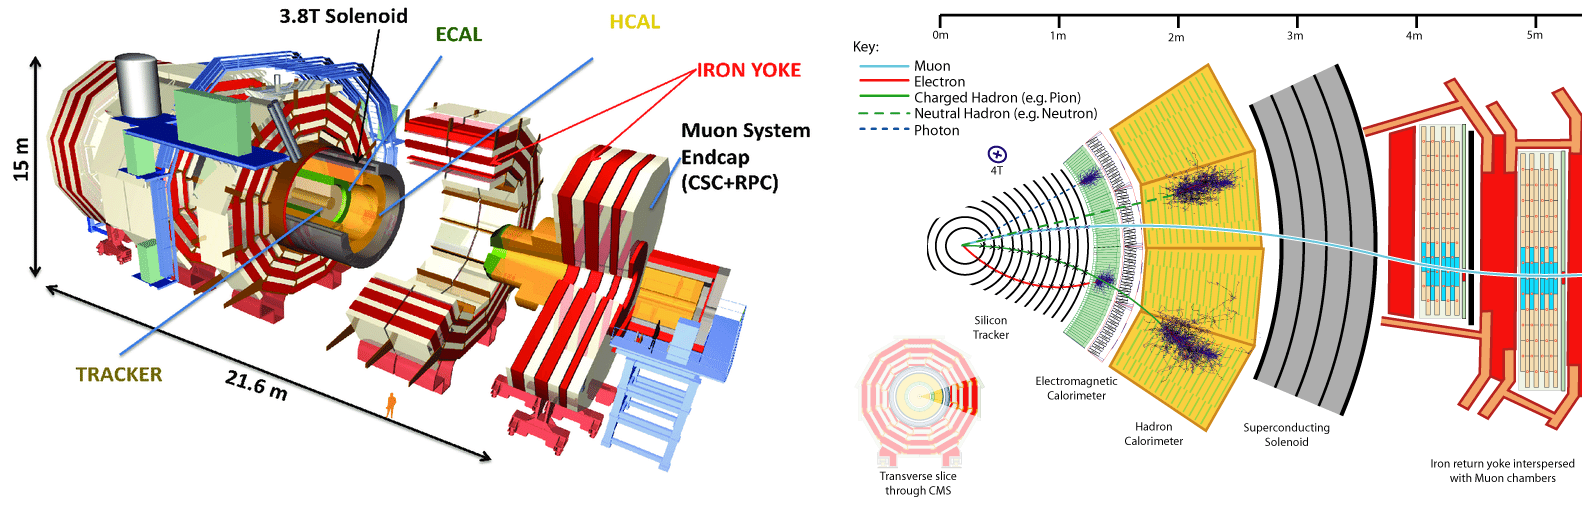
\includegraphics[width=1\columnwidth]{./cmsdetector_merged.png}
  \caption{Left: 3D design of CMS detector showing various concentric layers. Right: \onehalfspacing Transverse view of the CMS detector showing the silicon tracker, electromagnetic calorimeter, hadron calorimete##r, superconducting solenoid and muon chambers. \cite{Chatrchyan:2008aa}}
  \label{fig:CMSdetector}
\end{figure}





\subsection{The Pixel detector}

The pixel detector is the innermost of CMS tracker that contains 60 million pixels and these pixels assist in tracking the paths of particles emerging from the collision point. It is the nearest detector to the beam pipe and so will be vital in reconstructing the tracks of very short-lived particles. As it is very close to the collision point which means that the number of particles passing through is huge, the rate of particles received at 8cm from the beam line will be around 10 million particles per square centimetre per second. This feature is used to calculate the instantaneous luminosity $(L_{inst})$ by counting the number of pixel clusters which are collection of pixels hit by a track. The pixel detector is able to disentangle and reconstruct all the tracks left by the particles coming from the interaction point and has a long duration of 10 years. \\

The CMS Run 2 pixel detector consists of four concentric barrel layers (L1-L4) at radii of 29, 68, 109 and 160 mm and three disks (D1-D3) on each end at distances of 291, 396, and 516 mm from the center of the detector. It is built from 1856 segmented silicon sensor modules, where 1184 modules are used in the barrel pixel detector (BPIX) and 672 modules are used for the forward disks (FPIX) \cite{TrackerGroupoftheCMS:2020bgg}. \\

Each layer of the pixel detector is spilt into tiny square segments with each segment containing a silicon sensor having dimensions 100$\mu$m $\times$ 150$\mu$m as shown in the right part of Fig. 5. When a charged particle passes through this silicon sensor, it transfers energy to silicon atoms which causes electrons to be ejected from it creating electron-hole pairs. Each pixel uses an electric current to collect these charges on the pixel surface as a small electric signal. A electronic silicon chip is attached to each segment which amplifies the signal. The particle trajectory is deduced by knowing the hit pixels and as the pixel detector is made of two dimensional segments with four layers, we can create a three-dimensional picture of the path taken by the charged particle.



\begin{figure}[H]
  \centering
  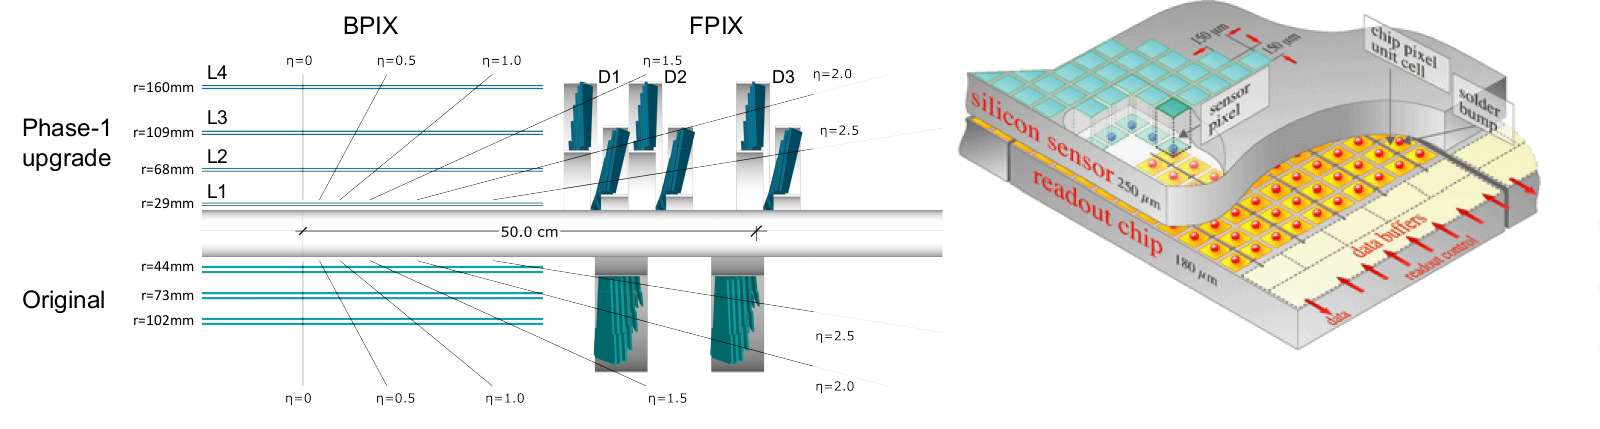
\includegraphics[width=1 \columnwidth]{./pixeldetector_merged1.png}
  \caption{Left: Layout of the CMS Run 2 pixel detector compared to the original detector layout, in longitudinal view. Right: pixel detector diagram showing size of Silicon sensor, readout chip and data buffers.}
  \label{fig:LHC}
\end{figure}




\section{The Pixel Cluster Counting (PCC) method}
\label{sec:pcc}
(describe cluster reconstruction, the module selection/veto, cluster counting per bx, per LS,..) \\

Pixel cluster counting (PCC)  method is an offline technique for the calculation of instantaneous luminosity $(L_{inst})$ for any LHC run period by counting the number of pixel clusters in the pixel detector (innermost segment of the CMS tracker) in a zero bias event which requires that only two bunches cross at the CMS interaction point. The mean number of pixel clusters can be expressed in terms of mean number of pixel clusters per proton-proton interaction and the number of proton-proton interaction per bunch crossing that is also called pileup (PU). \\

$<N_{cluster}>$ = $<N_{cluster/interaction}>$ (PU)  or (PU) = $\frac{<N_{cluster}>}{<N_{cluster/interaction}>}$ \\

The instantaneous luminosity per bunch crossing $L_{inst/bunch}$ is proportional to the number of proton-proton (pp) interactions per bunch crossing (pileup) and the proportionality constant is the ratio of  LHC orbit frequency f and the pp interaction cross section $\sigma_{interaction}(\sqrt{s})$ where s is the proton-proton collision center-of-mass energy \cite{CMS-PAS-LUM-12-001}. \\

$L_{inst/bunch}$ = $\frac{f}{\sigma_{interaction}}$ (PU)  \\

$L_{inst/bunch}$ = $\frac{<N_{cluster}> \: f }{<N_{cluster/interaction}> \: \sigma_{interaction}(\sqrt{s})}$ \\

The PCC visible cross section $\sigma_{vis}$ which is a calibration constant between pixel clusters rate and luminosity can be defined as \\

$\sigma_{vis}$ = $<N_{cluster/interaction}>$  $\sigma_{interaction}(\sqrt{s})$ \\

\newpage Thus, instantaneous luminosity per bunch crossing is given by \\

$L_{inst/bunch}$ = $\frac{<N_{cluster}> \: \sigma_{interaction}(\sqrt{s}) \: f }{ \:\sigma_{vis} \: \sigma_{interaction}(\sqrt{s})}$ \\

$L_{inst/bunch}$ = $\frac{<N_{cluster}> \:\: f}{\sigma_{vis}}$ \\

The PCC visible cross section $\sigma_{vis}$ is determined using van der meer scan method which is described in section 5. Cluster counting can be done over different time periods like 1 bunch crossing (25ns), 1 Lumi section (23.36s), 4 Lumi nibble (1.46s) and similarly instantaneous luminosity can be calculated over these time periods using PCC method. \\

LHC 2018 run can be categorized as follows, \\

1. Run2018A \\

Run number ranges from 315255 to 316995 \\
Number of runs per period is 146 \\

2. Run2018B\\

Run number ranges from 317080 to 319311\\
Number of runs per period is 132\\

3. Run2018C \\

Run number ranges from 319337 to 320065\\
Number of runs per period is 88 \\

Modules which are observed to function efficiently are considered for luminosity calculation. The module veto lists correspond to second Run2018D and select each detector part L2, L3, L4, D1, D2 and D3. Barrel layer 1 (L1) is not used for luminosity determination \cite{vetolist}. \\

1. veto lateRunD lowcut tight   (Number of vetoed modules 1387) \\
2. veto lateRunD lowcut tight B1 (Number of vetoed modules 1850)\\
3. veto lateRunD lowcut tight B2 (Number of vetoed modules 1766)\\
4. veto lateRunD lowcut tight B3 (Number of vetoed modules 1641)\\
5. veto lateRunD lowcut tight F1 (Number of vetoed modules 1813)\\
6. veto late RunD lowcut tight F2 (Number of vetoed modules 1799)\\
7. veto late RunD lowcut tight F3 (Number of vetoed modules 1800)\\

Specific techniques are employed for the reconstruction of clusters in the pixel detector and all the reconstructed clusters are used for counting to calculate the instantaneous luminosity. Algorithm used for finding clusters check for pixels whose signal to noise ratio is more than 6 and then merge adjacent pixel. These algorithms estimates cluster position in two directions and cluster charge. A cluster is a set of adjacent pixels and only pixels above certain minimum value of charge are considered. Position of a cluster in X and Y directions are obtained by fitting X and Y projections to templates that are estimates for cluster shapes \cite{Chatrchyan:2014fea}. \\


\begin{figure}[H]
  \centering
  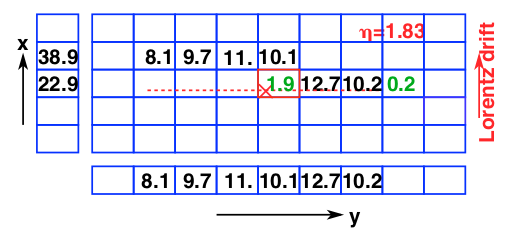
\includegraphics[width=0.6\columnwidth]{./pixel_reco.png}
  \caption{ \onehalfspacing Diagram showing pixel cluster with charge accumulation in each pixel expressed in terms of thousands of electrons. Green numbers represent charge accumulation below the 2000 electron threshold which are excluded clusters. The dotted red line indicates the particle trajectory projection in the module plane and the red cross shows the position of true hit.}
  \label{fig:CMS}
\end{figure}










\section{van der Meer calibration}
\label{sec:vdm}


\newpage \section{Backgrounds}
\label{sec:bkg}
(background in vdM, afterglow backgrounds in Physics, subtraction of these) \\

N= \sigma \:L + N_{background} \\

L = $ \int L_{inst} \: dt = \int \frac{R(t)}{\sigma_{vis}} \:dt $  \\

\sigma = \sigma_{interaction} (\sqrt{s}) \: A \:\epsilon\\

N: total number of event including signal and background. \\

$R(t) = \frac{d}{dt} <N_{cluster}>$ is the time dependent cluster rate. \\

$N_{background}$: Number of background events \\

$\sigma_{vis}$: PCC visible cross section.\\

$\sigma_{interaction}$ : proton-proton interaction cross section. \\

s: center of mass energy of colliding protons. \\

A: acceptance of the pixel detector. \\

$\epsilon$ : efficiency of the pixel detector. \\

$L_{inst}$: instantaneous luminosity.\\

The pixel cluster counting (PCC) method produces a small out-of-time response (OOTR, or ‘afterglow’) that has two types.\\

Type 1: fake hits in the bunch crossing after the colliding bunches (signal charge spillover).\\

Type 2: Activated material in the detector due to the large radiation doses, exponentially decays for many bunch crossings.\\

Afterglow effects are tiny in the case of tracklets (2x and 3x coincidences).\\

Due to both the late-arriving particles and energy originating from activated detector material, the pixel data need to be corrected for afterglow effects. This effect was studied in data taken using random triggers (triggers that fire randomly in bunch crossings spread over the whole LHC orbit except for the abort gap), considering the pixel cluster counts in bunch crossings after bunch trains. The resulting correction depends on the LHC filling scheme and for a typical 2011 fill with 1380 bunches corresponds to a subtraction of close to 2.8$\%$ of the integrated luminosity per luminosity section. \\

The afterglow corrections for PCC during 2017 run are in the range 2-5 $\%$ for the Type 1 corrections and 2-3 $\%$ averaged over all active bunches for the Type 2 corrections \cite{Sirunyan:2759951}.

\begin{figure}[H]
  \centering
  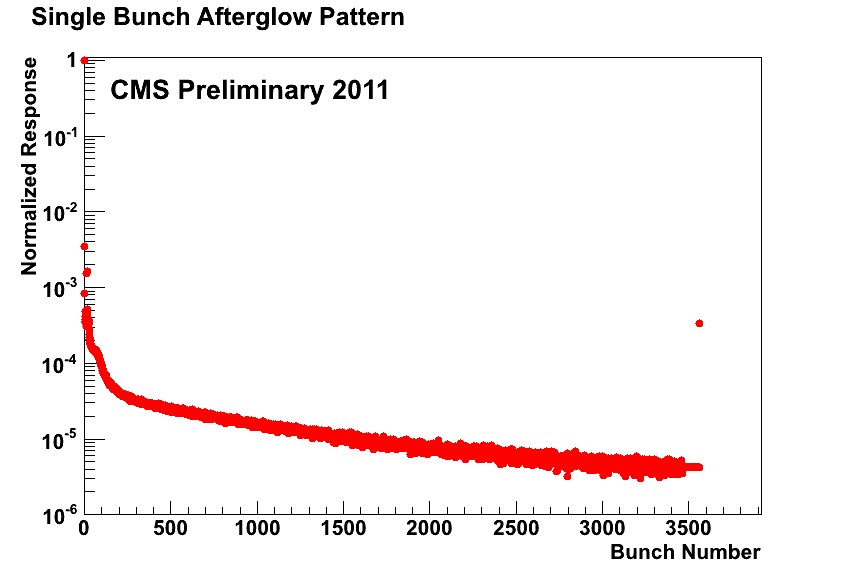
\includegraphics[width=0.5\columnwidth]{./SingleBunchAfterglow.png}
  \caption{Afterglow effect produced by a single colliding bunch.}
  \label{fig:LHC}
\end{figure}


Fig. 7 shows the afterglow noise induced by one colliding bunch. Since it is normalized to 1 at the first bin it means the first bin is the colliding bunch. The values at bins $>$ 1 are the cluster counts observed for bunches after the colliding bunch divided by the cluster counts observed by the colliding bunch. There are three parts to this distribution: \\

bin 1: colliding bunch \\

bin 2 (empty bunch): bunch after colliding bunch, noise observed is due to electronics signal on same pixels from colliding bunch. This is called Type 1. \\

bins $>$ 2 (empty bunches): noise observed is due to "albedo" which is material activated by the radiation of the collisions, it decays exponentially with time just like radioactive material. It produces secondary particles which create hits late in time. This is called Type 2.

\begin{figure}[H]
  \centering
  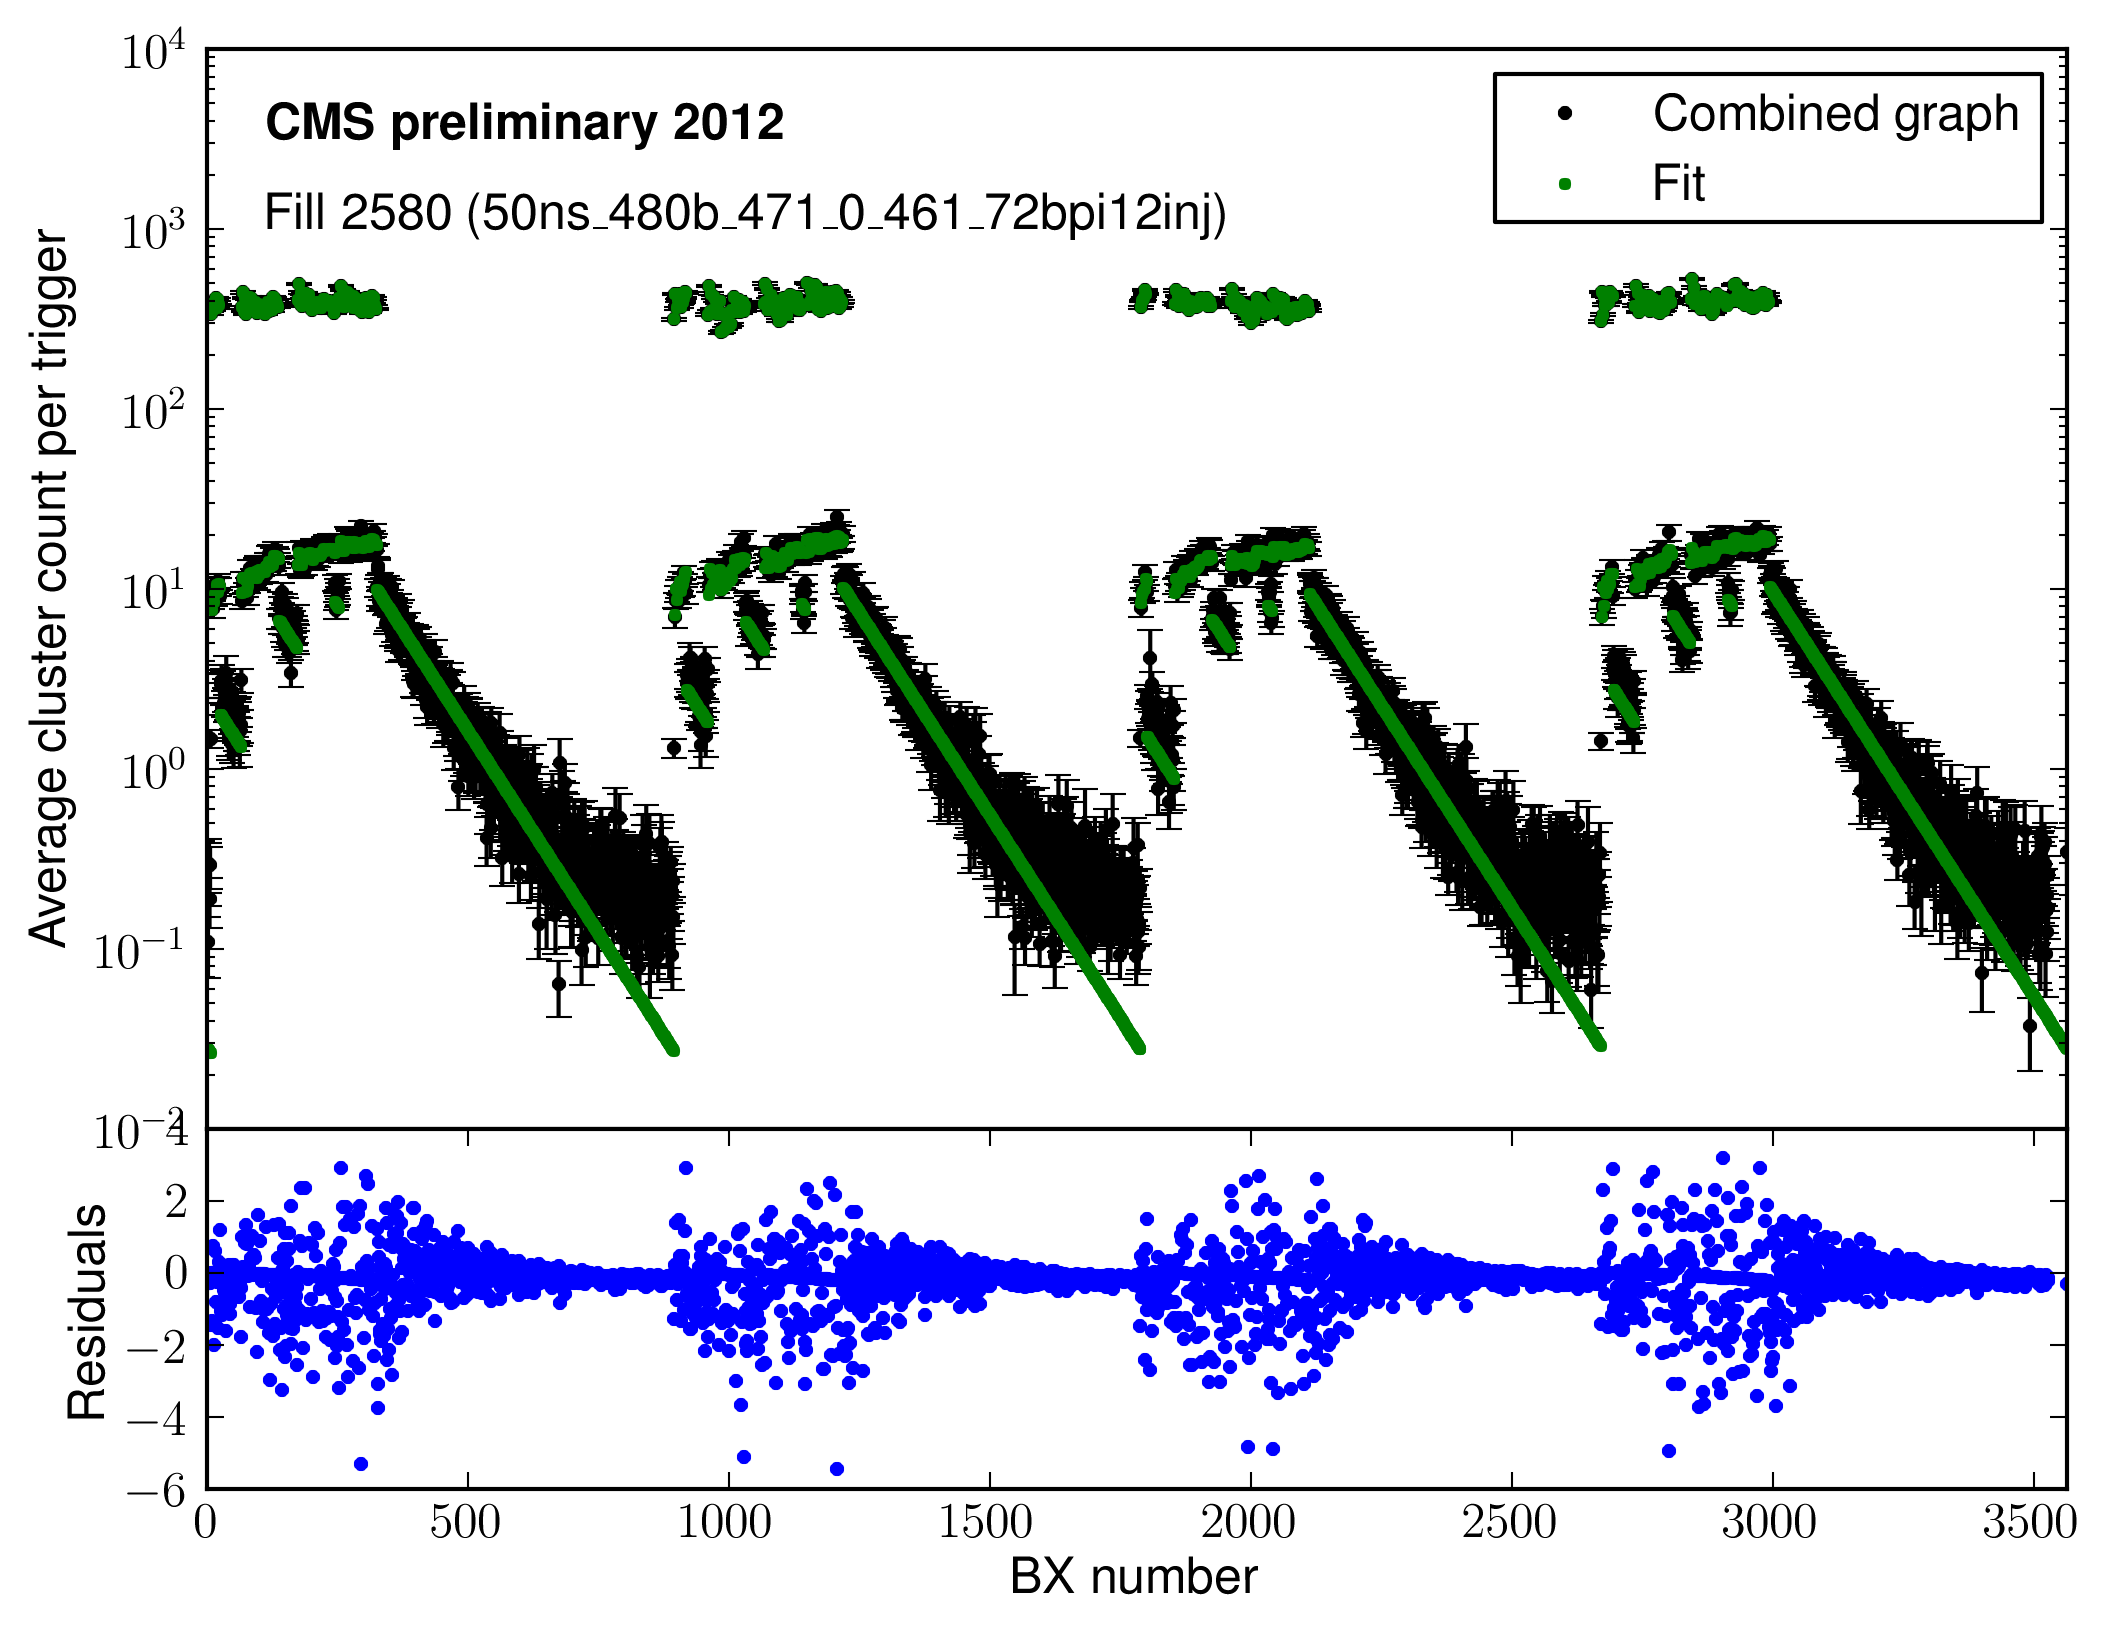
\includegraphics[width=0.5\columnwidth]{./afterglow.png}
  \caption{Results of the pixel afterglow 'deconvolution fit'}
  \label{fig:LHC}
\end{figure}


\begin{figure}[H]
  \centering
  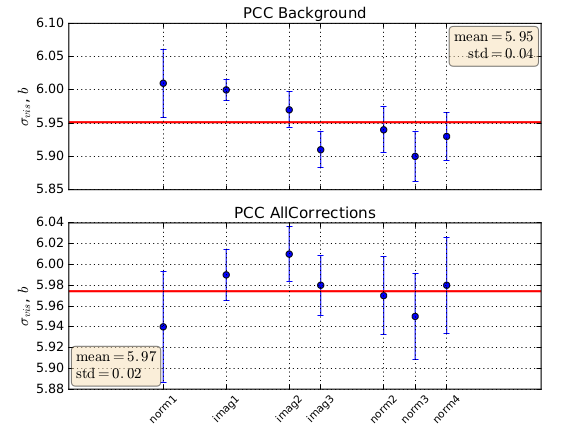
\includegraphics[width=0.6\columnwidth]{./PCC_background.png}
  \caption{ \onehalfspacing \cite{}.}
  \label{fig:CMS}
\end{figure}


\section{Systematics}
\label{sec:syst}
(main systematics: vdM, non-linearity, stability, check others in the PAS) \\

Systematic uncertainties in the beam overlap widths along x and y directions measured during vdM scans, $\sigma_{vis}$ and CMS luminosity can arise from length scale calibration, orbit drift, XY correlations of beam proton density distribution function, emittance growth, beam-beam deflection, dynamic $\beta$ which tells us whether bunches are narrow or wide, beam current calibration, ghosts and satellites, scan to scan variation and bunch to bunch variation. Systematic uncertainty during physics runs (high pileup) can be due to cross-detector consistency, afterglow effects, linearity and CMS deadtime. \\

\textbf{Systematics uncertainties during vdM scans or in $\bf{\sigma_{vis}}$:} \\

1. Length scale calibration: Acurracy of the beam positions from the LHC magnetic currents is limited that is why length scale calibration is done in which beams are moved in forward and backward directions at constant separation. A linear fit between the measured position and nominal position is plotted and deviation of the slope of this curve from one is used as correction. \\

2. Emittance growth: Beam size is known to increase during the fill which affects the cluster rate profile amplitude, its width and luminosity. Their variation is studied as a function of time and a linear fit is performed to obtain correction. Effect is sizable during a period of 30 minutes. \\

3. Orbit drift: Beams can slowly drift from their nominal positions in the transverse plane which causes beam separation to vary over a period of vdM scan step. LHC beam position monitoring systems are used to correct for beam separation. \\

4. XY correlations: The vdM scan method assumes that the shape of the bunch proton density function is factorizable into independent X and Y dependent terms which is not fully true and can lead to a biased estimate of the bunch overlap area $\Sigma_x \Sigma_y$. In order to measure this effect, special beam imaging scans are conducted in which one beam is fixed and other beam is moved across. In these scans, the measured vertex position distributions are used to derive the beam proton densities where Super Double Gaussian function is used as best fit and correction to the visible cross section $\sigma_{vis}$ is estimated. \\

5. Beam-Beam Effects: \\

Dipolar kick (beam-beam deflection): Repulsive force due to beam's electric field deflects other beam which affect nominal separation, the beam width and beam current. \\
Quadrupolar defocusing (dynamic $\beta$): Beam can get defocused by other beam's magnetic quadrupole field. Effective beam width is modified depending on the separation which in turn affects the peak instantaneous luminosity value because collision rate is decreased by 10 \%. \\

\newpage
\textbf{Systematics uncertaintities during physics runs (high pileup)}:\\

6. Non-Linearity: extrapolation of $\sigma_{vis}$ from vdM scans to high pileup physics data-taking periods can cause it to vary with per bunch instantaneous luminosity and pileup if the relation between luminosity and pileup is not linear.                               \\

7. Stability: Instability can arise from variation of measured cluster rate over time for different subdetectors in pixel detector and change of detector conditions over time for example detector noise, aging effects, radiation damage, etc. Results for PCC luminosity stability for 2018 data is described in the next section.                               \\

8. Cross-detector comparisons: After corrections of out-of-time effects and efficiency changes monitored by emittance scans, residual effects are evaluated by cross-detector comparison.                    \\

8. Afterglow effects: A small out of time response appears in unfilled bunches after colliding bunches. These effects are described in detail in the previous section \cite{CMS-PAS-LUM-18-002}. 





\newpage \section{Results}
\label{sec:results}

The stability of run 2018 CMS integrated luminosity for Phase I pixel detector calculated using PCC method is investigated by employing late Run2018D veto list.

\begin{figure}[H]
  \centering
  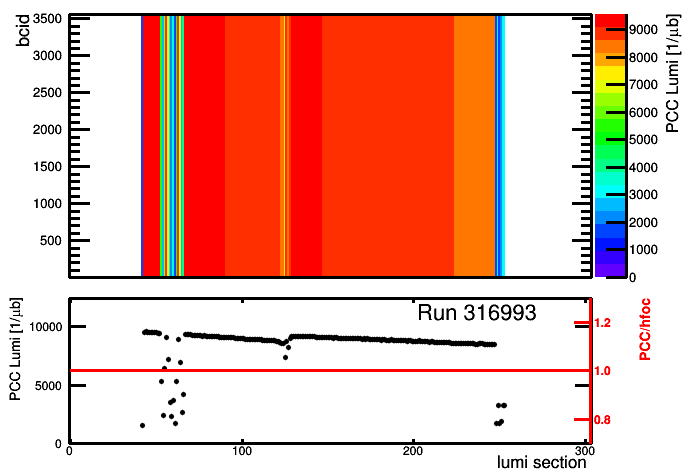
\includegraphics[width=0.52\columnwidth]{./316993.png}
  \caption{Top: Bunch crossing id (bcid) and PCC luminosity as a function of lumi section (1 lumi section is 23.36s). Bottom: PCC lumi as a function of lumi section using late run 2018D veto list for Run2018A.}
  \label{fig:CMS}
\end{figure}


\begin{figure}[H]
  \centering
  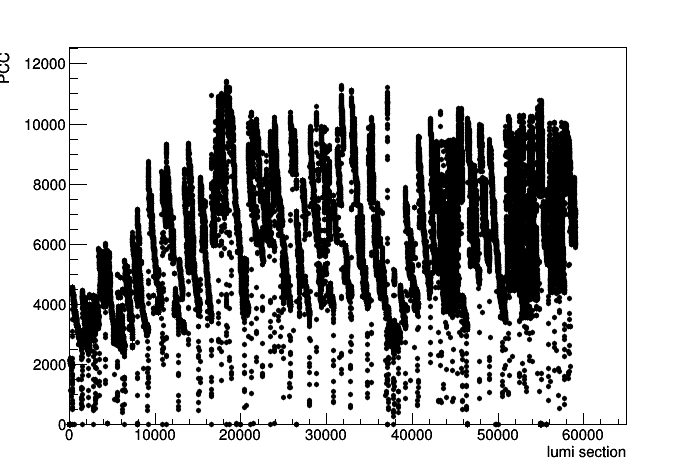
\includegraphics[width=0.52\columnwidth]{./ls_lumi.png}
  \caption{PCC luminosity ($\mu b^{-1}$) as a function of luminosity section (1 lumi section is 23.36s) for Run2018A.}
  \label{fig:CMS}
\end{figure}


\begin{figure}[H]
  \centering
  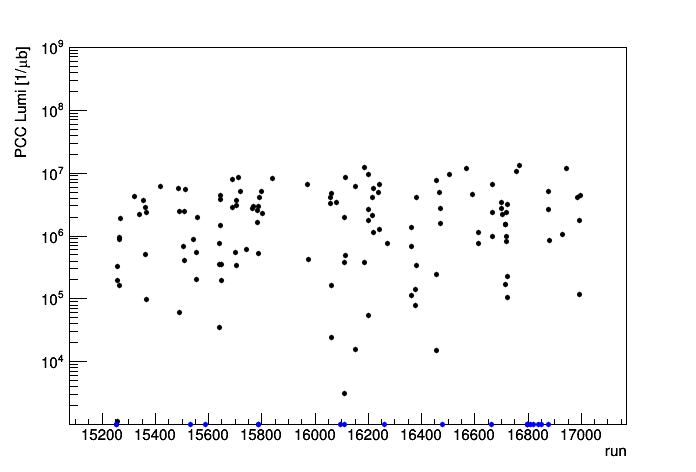
\includegraphics[width=0.52\columnwidth]{./runs.png}
  \caption{PCC luminosity ($\mu b^{-1}$) as a function of run number for Run2018A.}
  \label{fig:CMS}
\end{figure}


\begin{figure}[H]
  \centering
  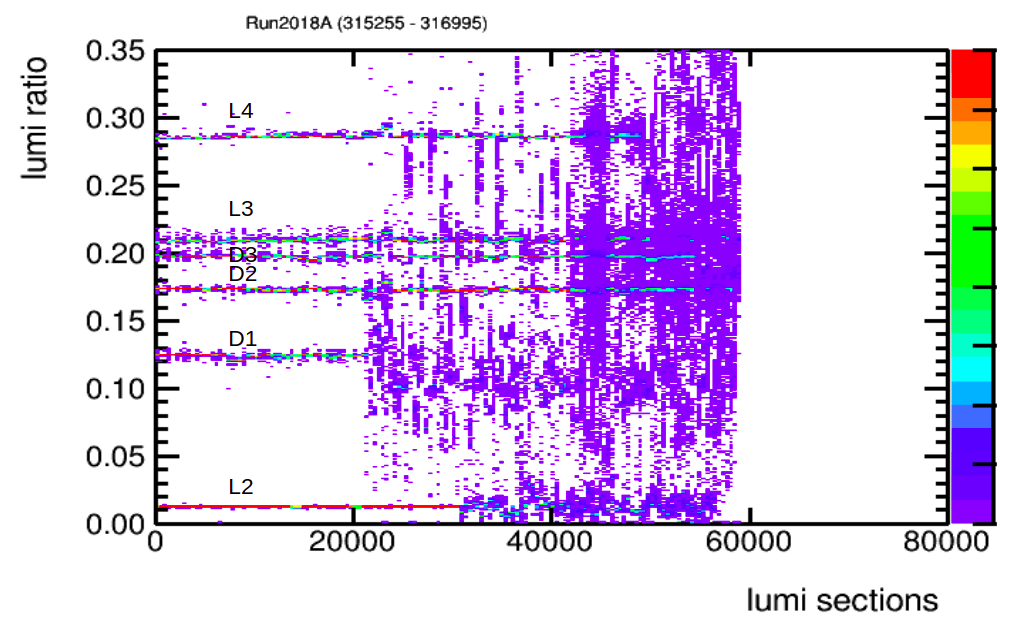
\includegraphics[width=0.52\columnwidth]{./2018A_lumiratio.png}
  \caption{Luminosity ratios for various subdetectors L2, L3, L4, D1, D2, D3 of pixel detector as a function of lumi section for Run2018A.}
  \label{fig:CMS}
\end{figure}



\begin{figure}[H]
  \centering
  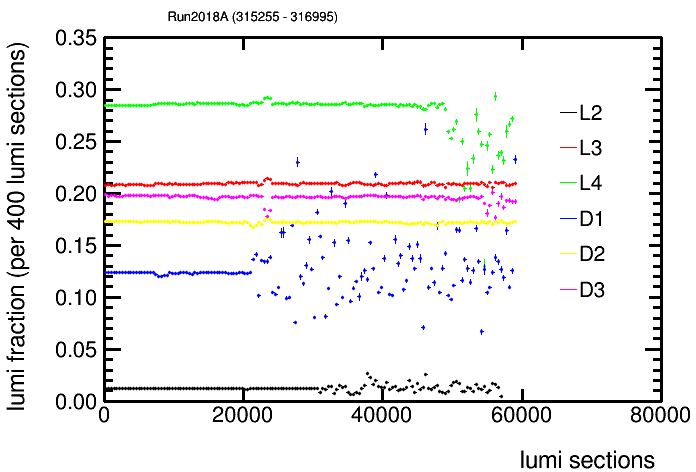
\includegraphics[width=0.52\columnwidth]{./ProfileXcombined_new.png}
  \caption{X Profile of luminosity ratios vs lumi section graph for various subdetectors L2, L3, L4, D1, D2, D3 of pixel detector showing luminosity fraction as a function of lumi section (1 lumi section is 23.36s) for Run2018A.}
  \label{fig:CMS}
\end{figure}





\begin{figure}[H]
  \centering
  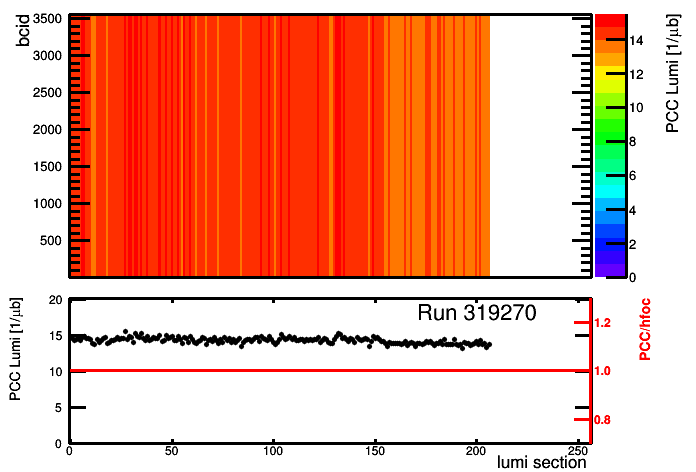
\includegraphics[width=0.52\columnwidth]{./319270.png}
  \caption{Top: Bunch crossing id (bcid) and PCC luminosity as a function of lumi section. Bottom: PCC lumi as a function of lumi section using late run 2018D veto list for Run2018B.}
  \label{fig:CMS}
\end{figure}


\begin{figure}[H]
  \centering
  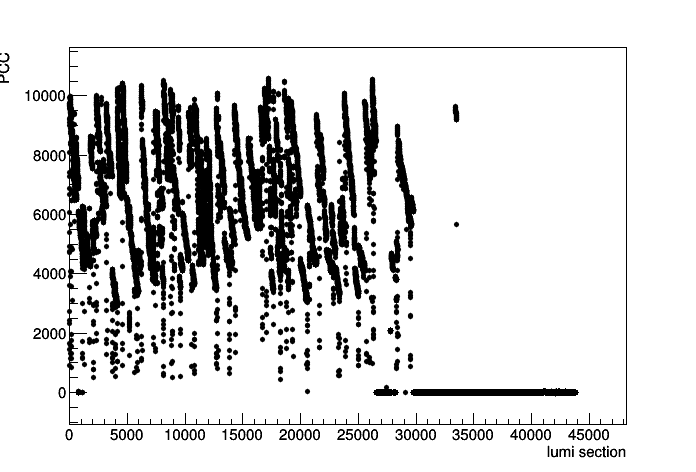
\includegraphics[width=0.52\columnwidth]{./ls_lumi_2018B.png}
  \caption{PCC luminosity as a function of lumi section for Run2018B.}
  \label{fig:CMS}
\end{figure}


\begin{figure}[H]
  \centering
  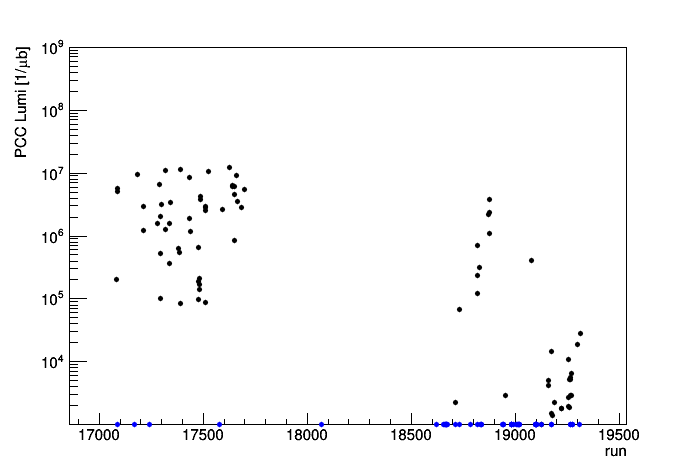
\includegraphics[width=0.52\columnwidth]{./runs_2018B.png}
  \caption{PCC luminosity as a function of run number for Run2018B.}
  \label{fig:CMS}
\end{figure}


\begin{figure}[H]
  \centering
  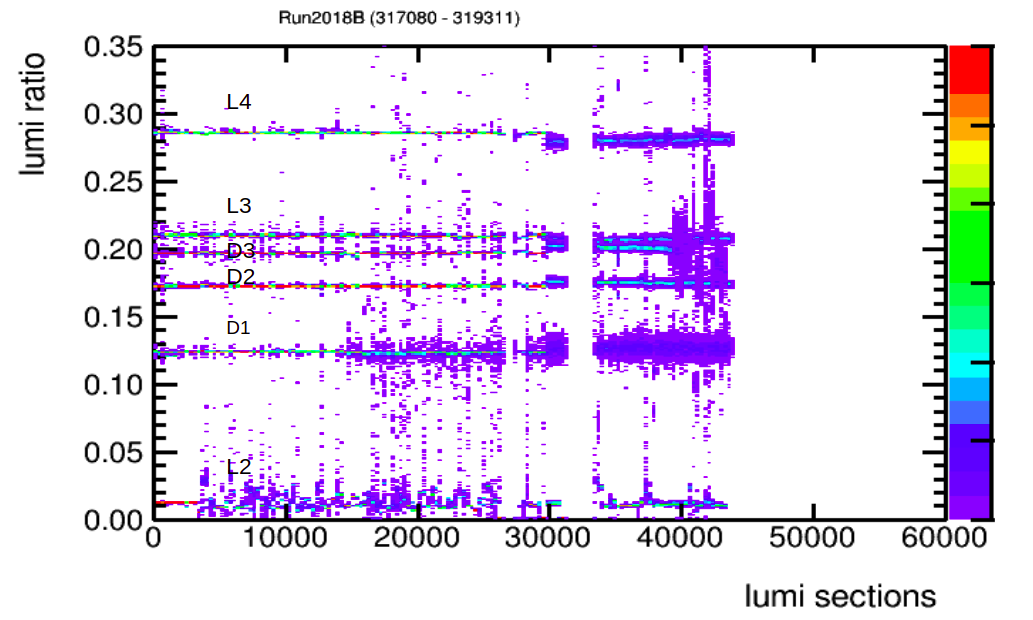
\includegraphics[width=0.52\columnwidth]{./2018B_lumiratio.png}
  \caption{Luminosity ratios for various subdetectors L2, L3, L4, D1, D2, D3 of pixel detector as a function of lumi section for Run2018B.}
  \label{fig:CMS}
\end{figure}



\begin{figure}[H]
  \centering
  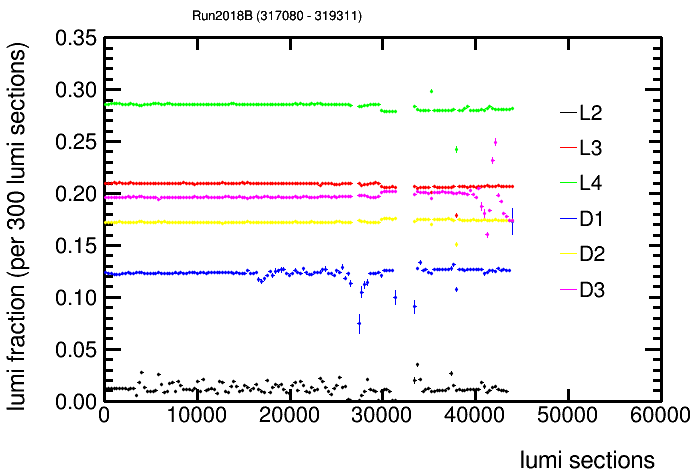
\includegraphics[width=0.5\columnwidth]{./ProfileXcombinedB_new.png}
  \caption{X Profile of luminosity ratios vs lumi section graph for various subdetectors L2, L3, L4, D1, D2, D3 of pixel detector showing luminosity fraction as a function of lumi section for Run2018B.}
  \label{fig:CMS}
\end{figure}



\begin{figure}[H]
  \centering
  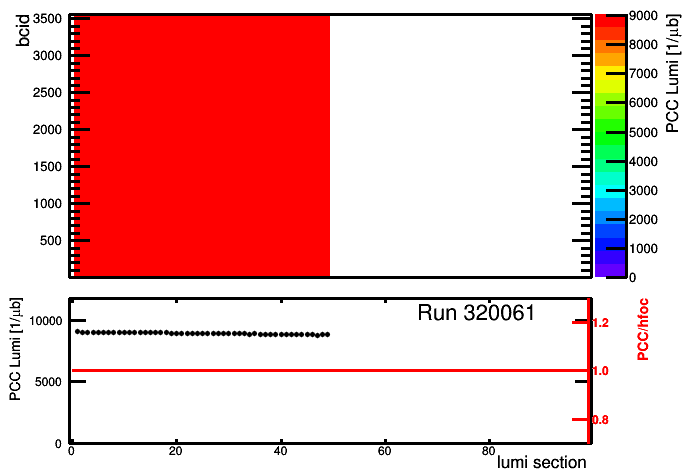
\includegraphics[width=0.5\columnwidth]{./320061.png}
  \caption{Top: Bunch crossing id (bcid) and PCC luminosity as a function of lumi section. Bottom: PCC lumi as a function of lumi section using late run 2018D veto list for Run2018C.}
  \label{fig:CMS}
\end{figure}


\begin{figure}[H]
  \centering
  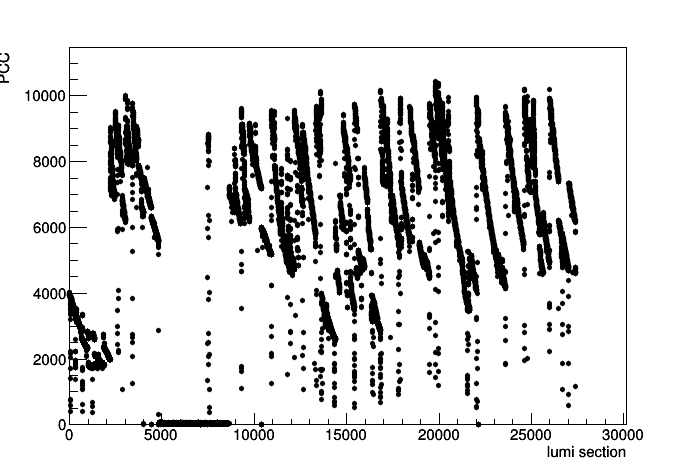
\includegraphics[width=0.5\columnwidth]{./ls_lumi_2018C.png}
  \caption{PCC luminosity as a function of lumi section for Run2018C.}
  \label{fig:CMS}
\end{figure}


\begin{figure}[H]
  \centering
  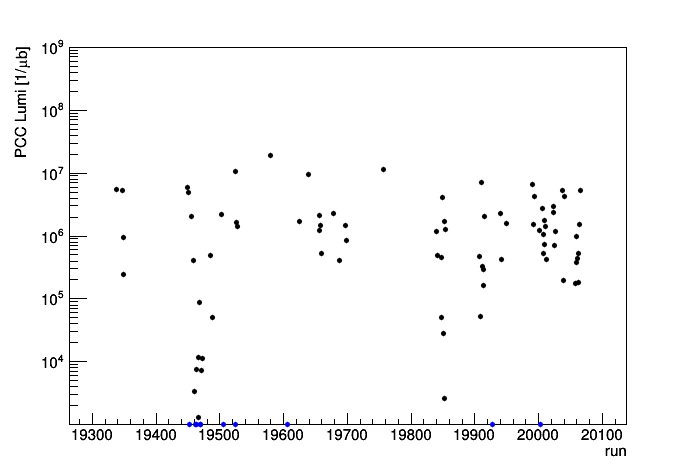
\includegraphics[width=0.5\columnwidth]{./runs_2018C.png}
  \caption{PCC luminosity as a function of run number for Run2018C.}
  \label{fig:CMS}
\end{figure}


\begin{figure}[H]
  \centering
  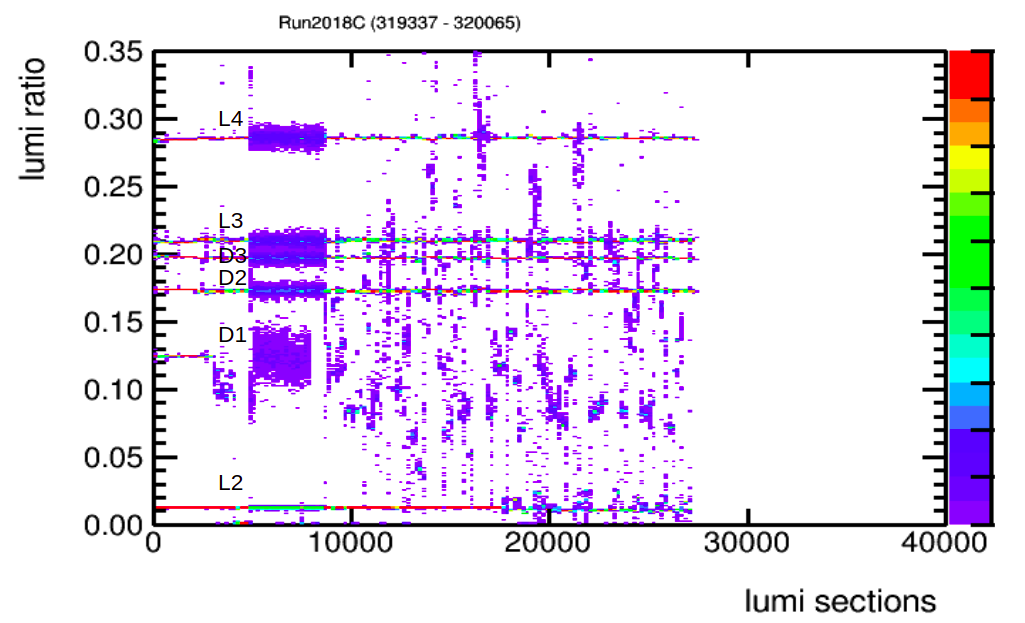
\includegraphics[width=0.5\columnwidth]{./2018C_lumiratio.png}
  \caption{Luminosity ratios for various subdetectors L2, L3, L4, D1, D2, D3 of pixel detector as a function of lumi section for Run2018C.}
  \label{fig:CMS}
\end{figure}


\begin{figure}[H]
  \centering
  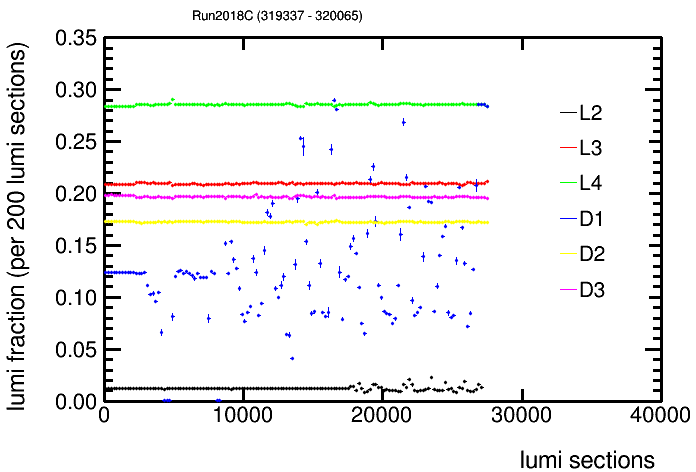
\includegraphics[width=0.5\columnwidth]{./ProfileXcombinedC_new.png}
  \caption{X Profile of luminosity ratios vs lumi section graph for various subdetectors L2, L3, L4, D1, D2, D3 of pixel detector showing luminosity fraction as a function of lumi section for Run2018C. \cite{lumidpg}}
  \label{fig:CMS}
\end{figure}



\newpage \section{The TEPX upgrade for HL-LHC}
\label{sec:tepx}
(describe the TEPX detector design, algorithms clusters/coincidences, D4R1 as HL-LHC luminometer, stat precision, linearity)\\

The High Luminosity (HL)-LHC will increase instantaneous luminosity to unprecedented value of $7.5 \times 10^{34} cm^{-2} s^{-1}$ which corresponds to 200 proton-proton collisions per bunch crossing (pileup). Run 2 pixel detector will not be able to handle the extreme radiation environment, resolve nearby particle tracks and operate properly to give a reliable estimate of the instantaneous luminosity for high pileup values. That is why it will be replaced by a new pixel detector which will be composed of three subdetectors: tracker barrel pixel detector (TBPX), tracker forward pixel detector (TFPX) and tracker endcap pixel detector (TEPX). TEPX will have better radiation tolerance, increased granularity, improved two-track separation, improved estimation of hit rate and statistical precision, extended tracking acceptance $|\eta|=4$ with Disk 4 Ring 1 operating as an independent luminometer \cite{Klein:2017nke}. \\

Tracker endcap pixel detector (TEPX) consists of four double disks per side (-Z and +Z) as shown in Fig. 27 with each double disk containing five rings as shown in Fig. 28 having 20, 28, 36, 44 and 48 modules respectively. One double disk has four surfaces with +Z side containing modules with even module number in front layers (L1 $\&$ L2) and modules with odd module number in back layers (L3 $\&$ L4) from Ring 1 to Ring 4 and for Ring 5, modules with odd module number in front layers and modules with even module number in back layers as shown in Fig. 29. For -Z side, four surfaces contain modules with odd module number in front layer and modules with even module number in back layer from Ring 1 to Ring 4 and for Ring 5, modules with even module number in front layer and modules with odd module number in back layer . \\


Instantaneous luminosity determination using PCC method for Phase 2 HL-LHC can be based on counting the number of clusters or coincidences. The innermost ring of the last disk of TEPX (D4R1) is located at 2.65 m away from the interaction point that is beyond the tracking acceptance ($|\eta = 4|$) and as this region has few tracking points, it can be solely used for the purpose of luminosity measurement by using the full available trigger rate and bandwidth.  Two fold coincidences are those hits which are created by the module overlap regions between various layers of one TEPX double disk. Two fold coincidences are better way to distinguish between a real hit and random electrical noise. They are more likely to be real hit than random electrical noise. Two fold coincidence in $\phi$ will involve modules overlapping in the same ring in front and back layers of one double disk as shown in top part of Fig. 30 and Fig. 31 while two fold coincidence in r will require modules overlapping between successive rings in the front (L1 $\&$ L2) and back layers (L3 $\&$ L4) of one double disk as shown in bottom part of Fig. 30. Luminosity calculated based on counting coincidences has an advantage over clusters that afterglow effects are tiny in the case of coincidences.  \cite{Collaboration:2706512} \\


Nonlinearity is one of the systematic uncertainty in the calculation of instantaneous luminosity using PCC and PCC visible cross section $\sigma_{vis}$. A linear relation between the number of clusters and pileup (PU) would imply that\\

$<N_{cluster/interaction}> = \frac{<N_{cluster}>}{(PU)} = \frac{\sigma_{visible}}{\sigma_{interaction} (\sqrt{s})}$ \\

$<N_{cluster}> =  \frac{\sigma_{visible}}{\sigma_{interaction}(\sqrt{s})} (PU)$ \\

\newpage Linearity indicates that the PCC visible cross section $\sigma_{vis}$ does not depend on the per bunch instantaneous luminosity (ideal luminometer). In ideal  scenario, $\sigma_{vis}$ is not dependent on pileup, but this a potential problem with the luminometer. A non-linear relation $<N_{cluster}> = \alpha (PU)^{\gamma}, \gamma \neq 1$ would add non-linear terms in the rate equation $R = \sigma L$  and cause $\sigma_{vis}$ to vary with the per bunch instantaneous luminosity and pileup values.


\begin{figure}[H]
  \centering
  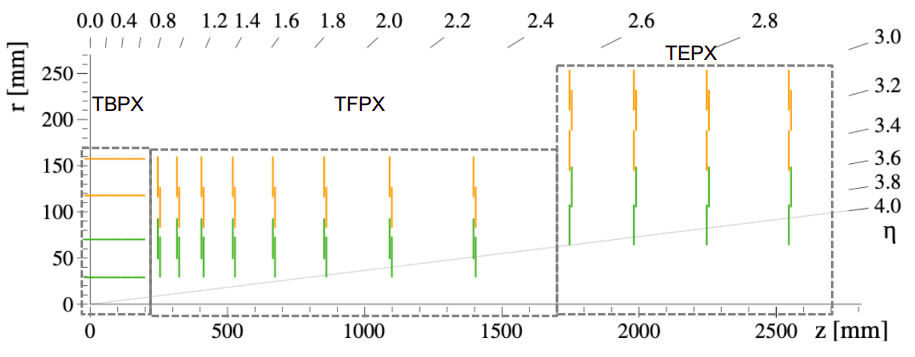
\includegraphics[width=0.8\columnwidth]{./tepx_geometry.png}
  \caption{ \onehalfspacing A layout of the CMS Phase-2 inner tracker showing four TEPX disks, eight TFPX disks and 4 barrel layers. \cite{Klein:2017nke}}
  \label{fig:CMS}
\end{figure}


\begin{figure}[H]
  \centering
  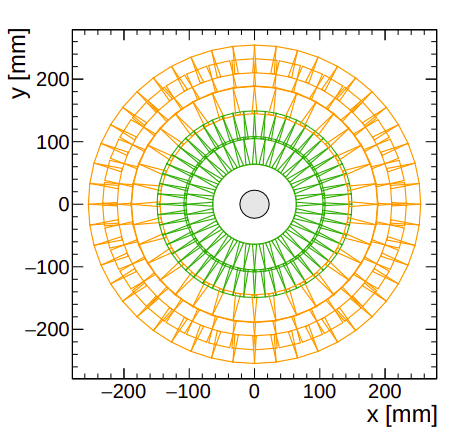
\includegraphics[width=0.5 \columnwidth]{./xydisc.png}
  \caption{ \onehalfspacing Sketch of the TEPX Disk layouts in x-y view. Modules of type 1 $\times$ 2 are shown in green, while 2 $\times$ 2 modules are represented in orange.}
  \label{fig:CMS}
\end{figure}

\begin{figure}[H]
  \centering
  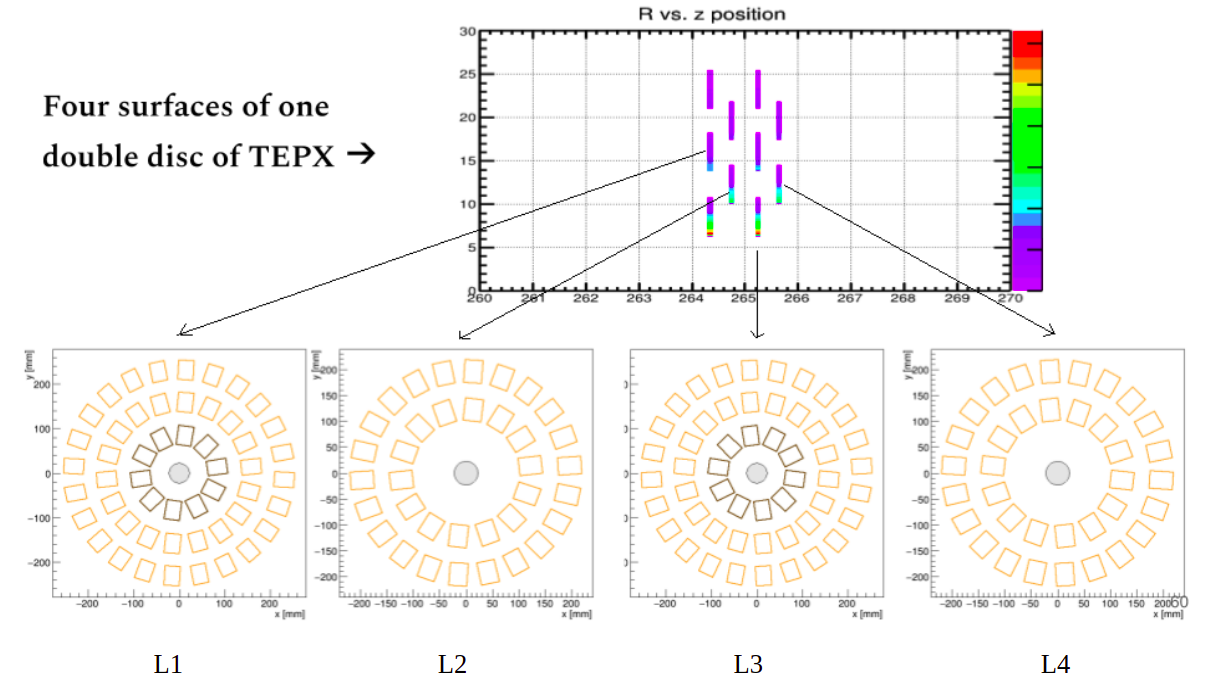
\includegraphics[width=1 \columnwidth]{./fourlayers.png}
  \caption{ \onehalfspacing Fours layers of one double disk of TEPX showing module arrangement in rings for all layers.}
  \label{fig:CMS}
\end{figure}




\begin{figure}[H]
  \centering
  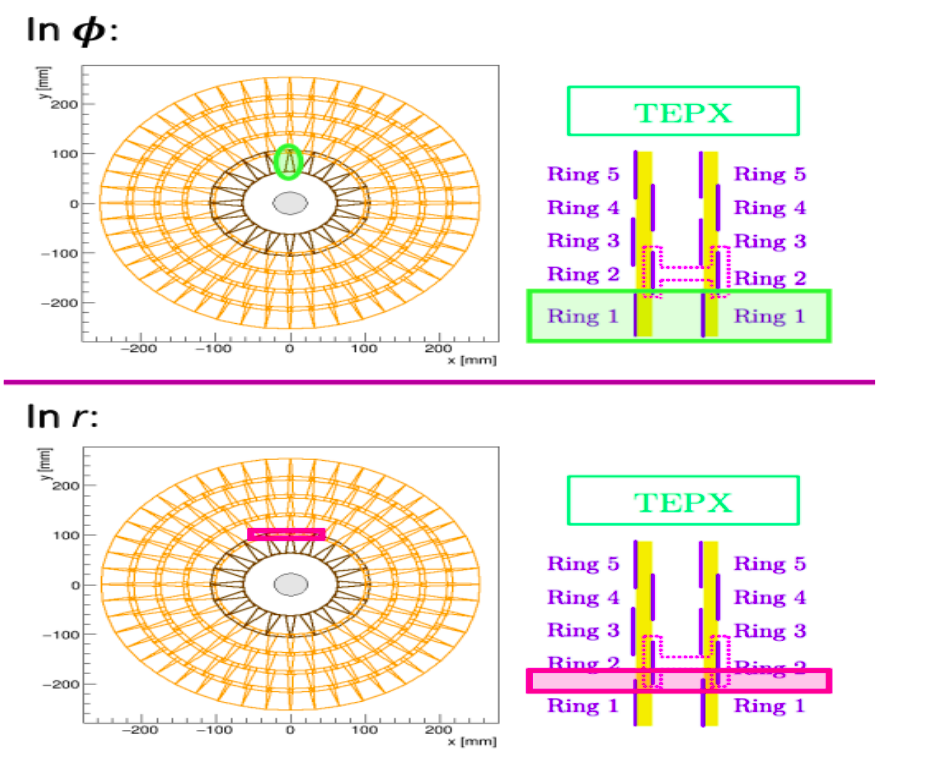
\includegraphics[width=0.8\columnwidth]{./coincidences.png}
  \caption{ \onehalfspacing Diagram showing modules overlap between the front and back layers of one double disk of TEPX that creates two fold coincidences in $\phi$ and r.}
  \label{fig:CMS}
\end{figure}

\begin{figure}[H]
  \centering
  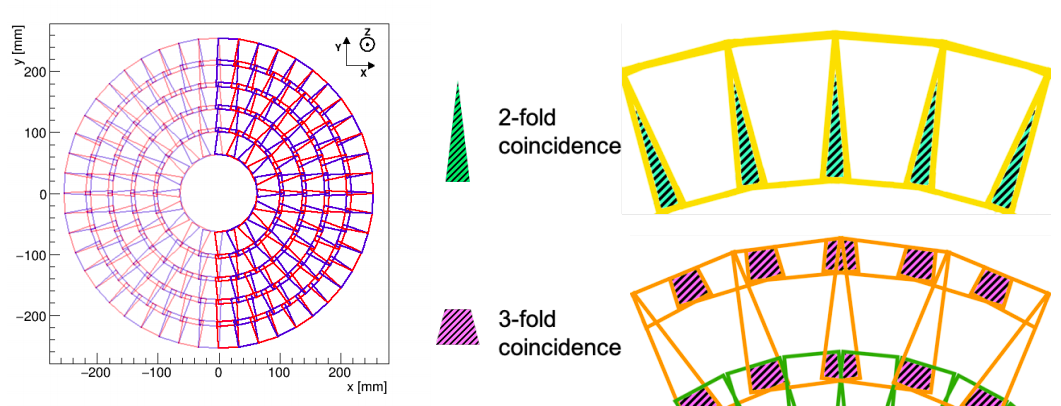
\includegraphics[width=0.8\columnwidth]{./up.png}
  \caption{\onehalfspacing Left: View in the x-y plane of the double disk structure of one TEPX disk. The sensors in blue and red correspond to the two double disks at slightly different z positions. Right: Example of two- and threefold coincidence regions on a portion of a single TEPX disk.}
  \label{fig:CMS}
\end{figure}


\newpage
\begin{figure}[H]
  \centering
  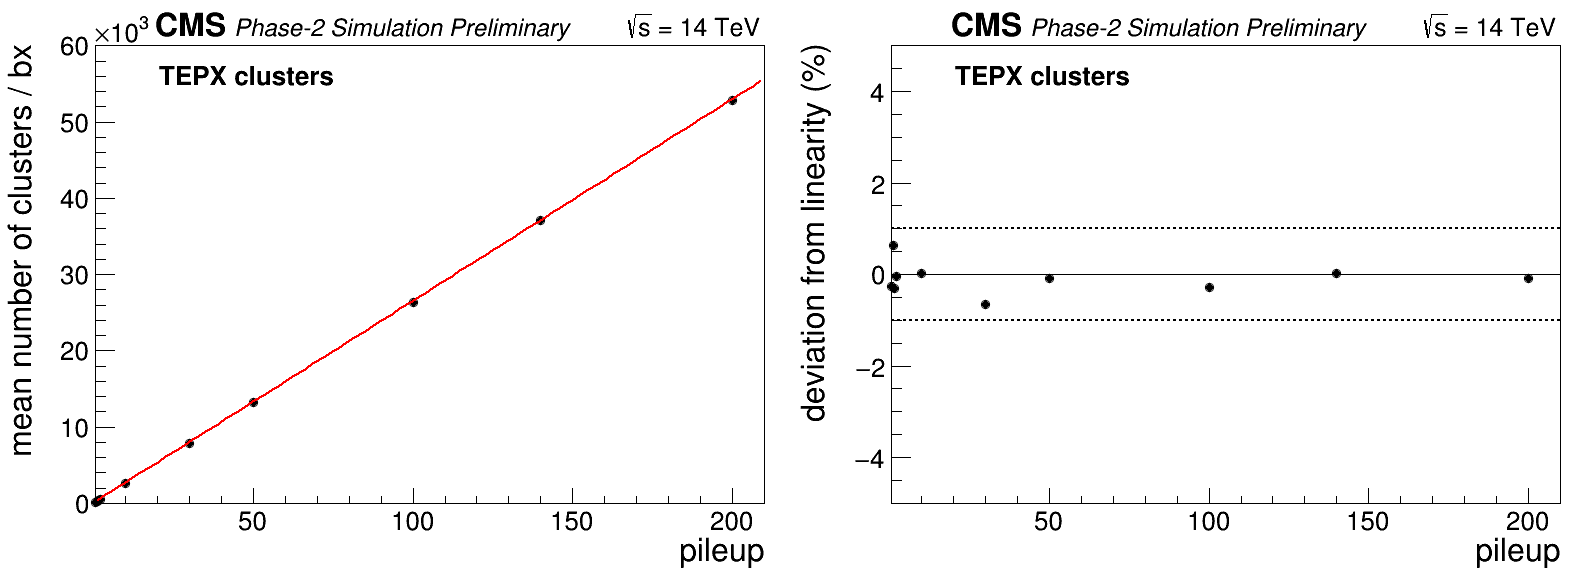
\includegraphics[width=1\columnwidth]{./totalclusters.png}
  \caption{\onehalfspacing Left: Simulated mean number of clusters for all entire TEPX detector as a function of pileup. A line is fitted between pileup values of 0 and 2, and then extrapolated up to a pileup of 200. Right: Deviation from linearity for clusters for entire TEPX detector. The non-linearity is calculated as the relative difference between the data points and the values of the fit function at the respective pileup value. Non-linearity is within 1 \% for entire pileup range. Pileup 200 corresponds to High Luminosity (HL)-LHC environment.}
  \label{fig:CMS}
\end{figure}



\begin{figure}[H]
  \centering
  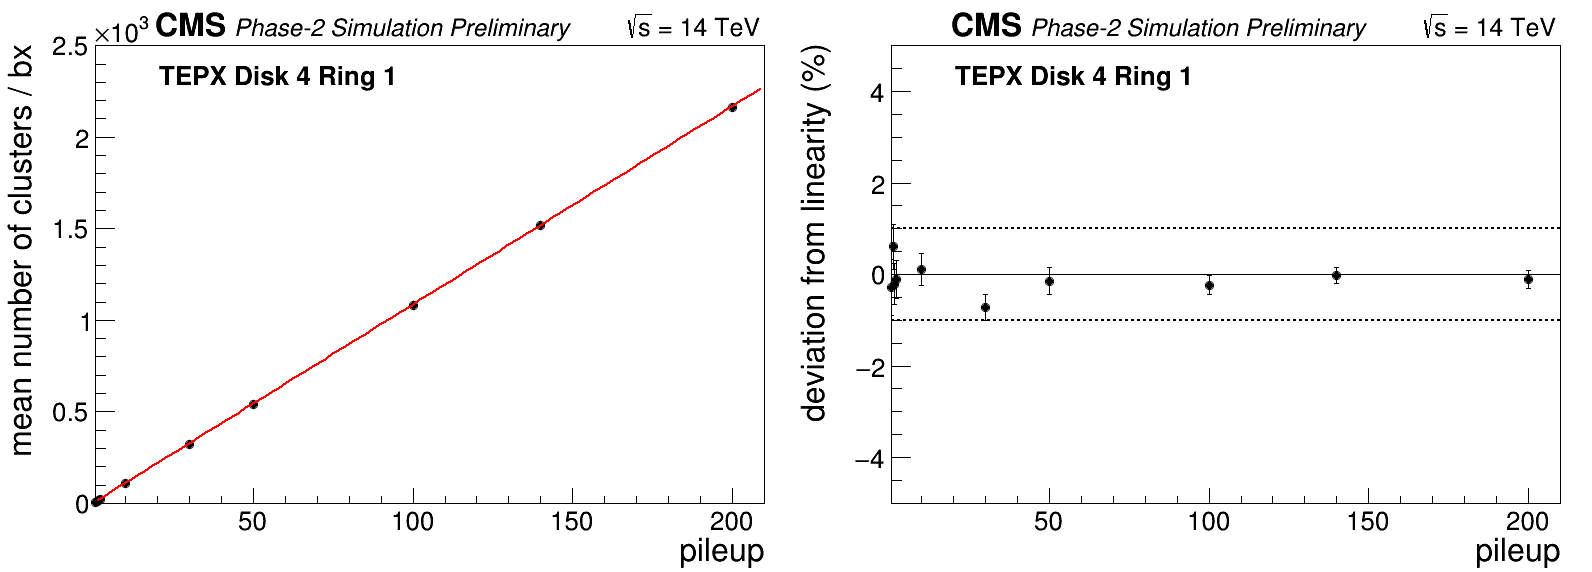
\includegraphics[width=1\columnwidth]{./clustersD4R1.png}
  \caption{\onehalfspacing Left: Simulated mean number of clusters for TEPX Disk 4 Ring 1 as a function of pileup. Right: Deviation from linearity for clusters for TEPX Disk 4 Ring 1. The non-linearity is calculated as the relative difference between the data points and the values of the fit function at the respective pileup value.}
  \label{fig:CMS}
\end{figure}



\begin{figure}[H]
  \centering
  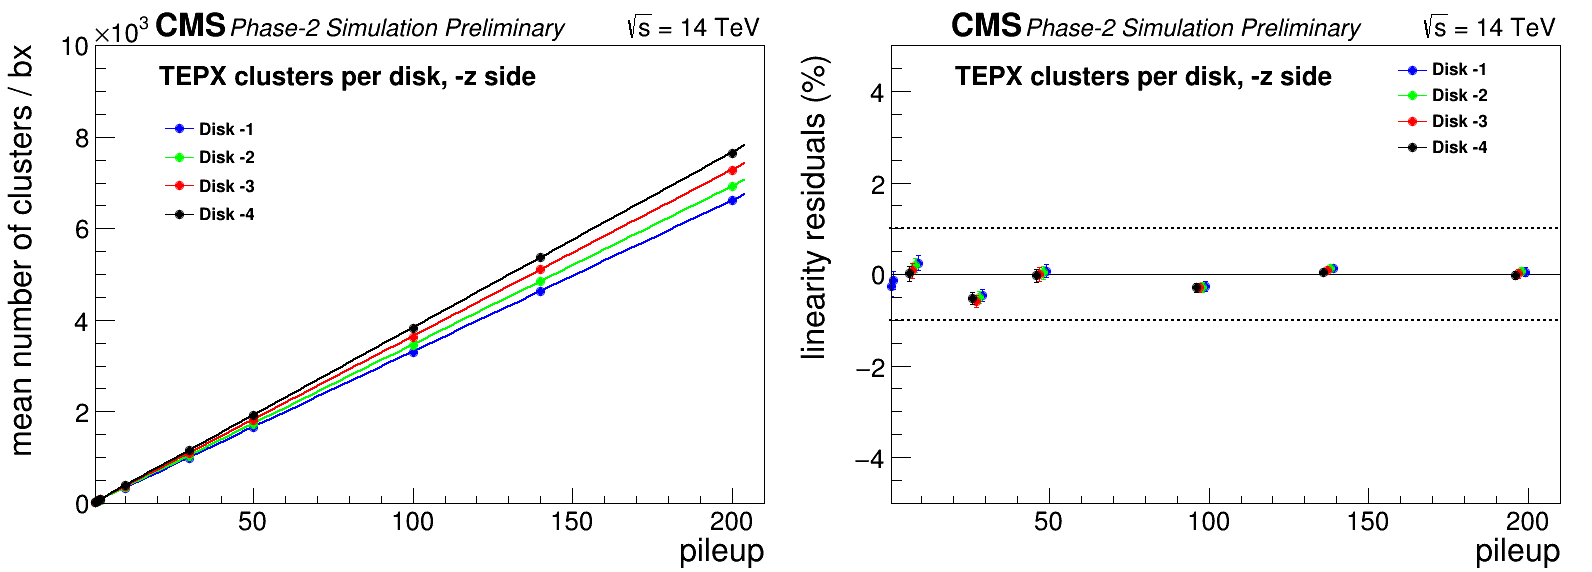
\includegraphics[width=1 \columnwidth]{./clustersperdisk-z.png}
  \caption{Left: Simulated mean number of clusters for -z side TEPX disks as a function of pileup. Right: Deviation from linearity for clusters for -z side TEPX disks.}
  \label{fig:CMS}
\end{figure}


\begin{figure}[H]
  \centering
  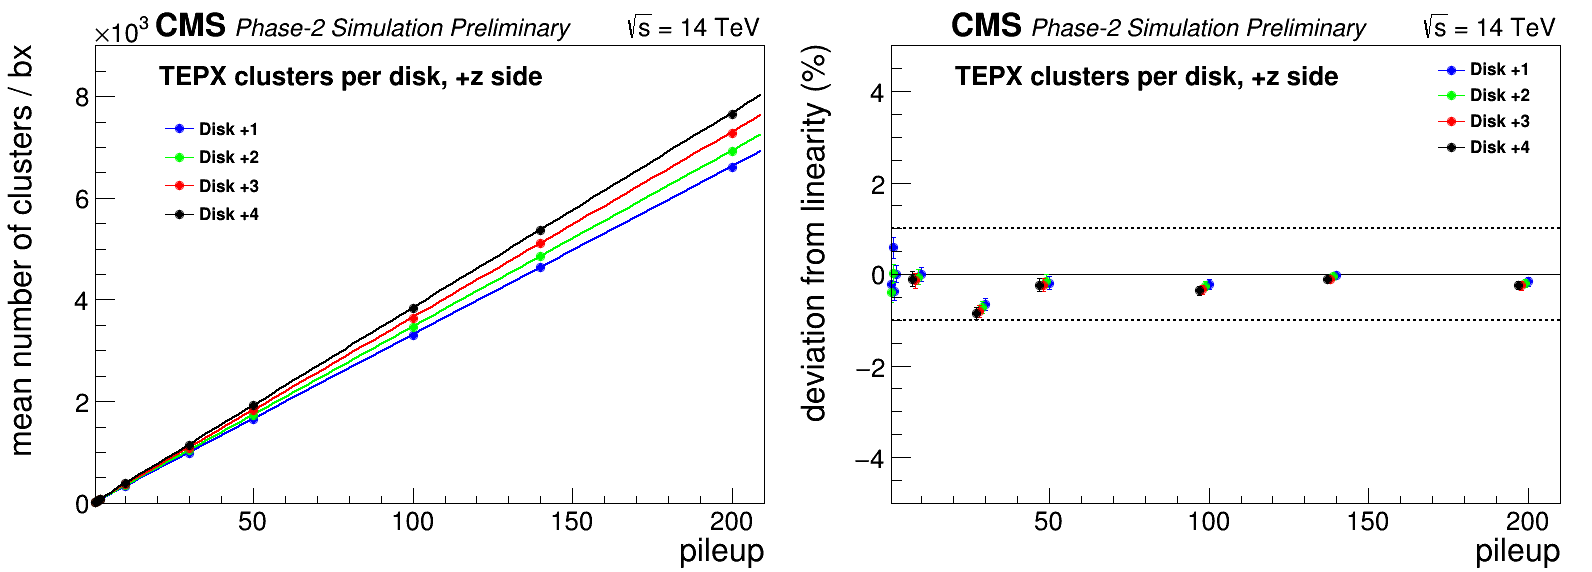
\includegraphics[width=1 \columnwidth]{./clustersperdisk+z.png}
  \caption{Left: Simulated mean number of clusters for +z side TEPX disks as a function of pileup. Right: Deviation from linearity for clusters for +z side TEPX disks.}
  \label{fig:CMS}
\end{figure}


\begin{figure}[H]
  \centering
  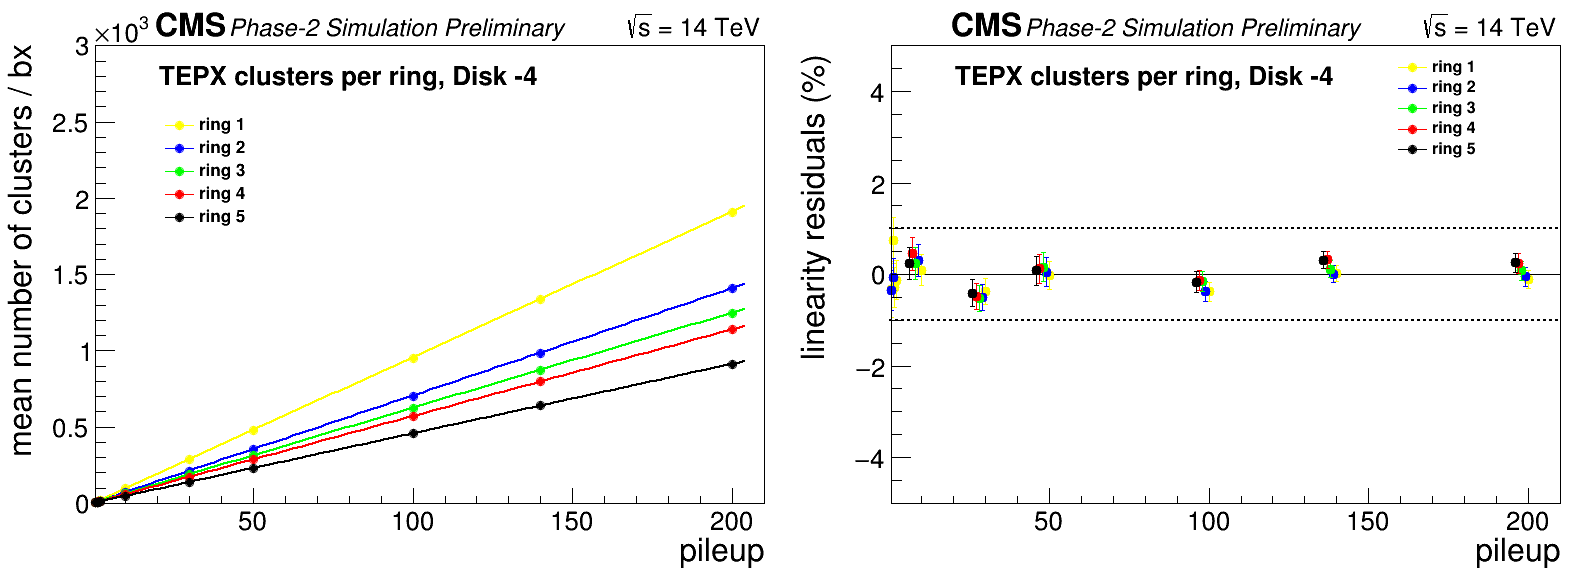
\includegraphics[width=1\columnwidth]{./clustersperringD-4.png}
  \caption{Left: Simulated mean number of clusters for TEPX Disk 4 all rings as a function of pileup. Ring 1 has highest slope and Ring 5 has least slope. Right: Deviation from linearity for clusters for TEPX Disk 4 all rings. Non-linearity is within $1\%$ for all rings over entire pileup range.}
  \label{fig:CMS}
\end{figure}

\begin{figure}[H]
  \centering
  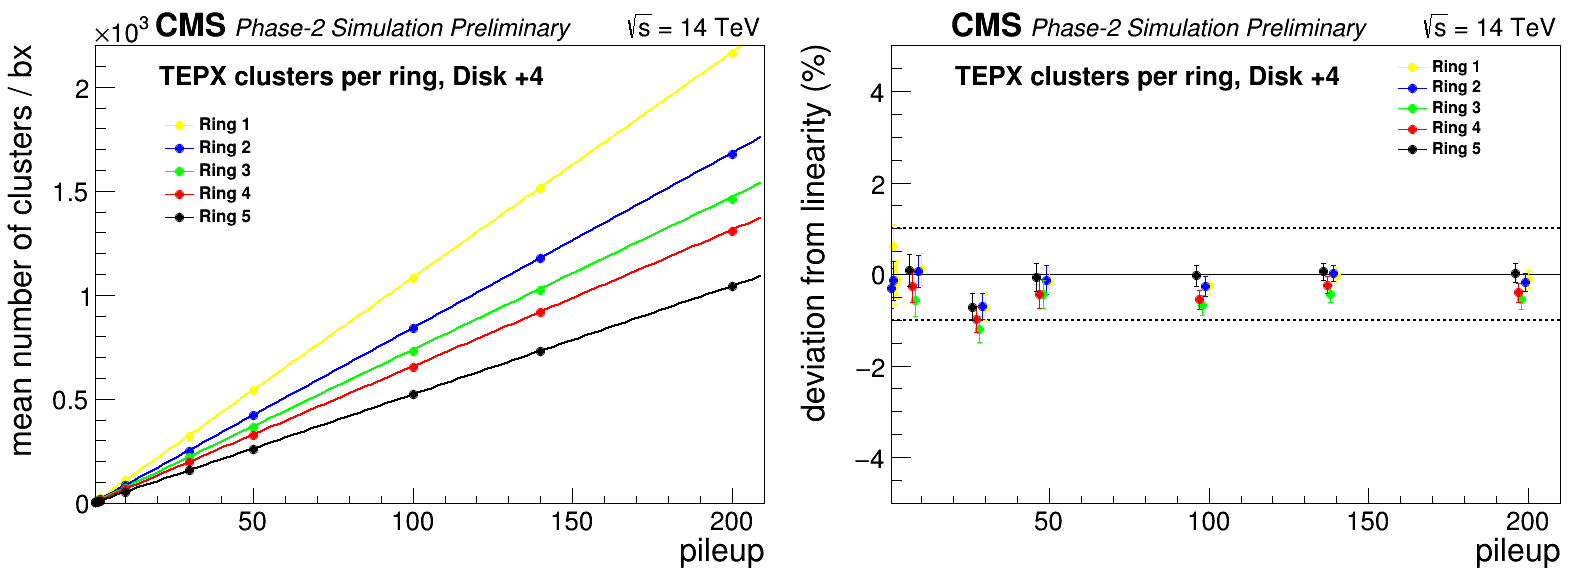
\includegraphics[width=1\columnwidth]{./clustersperringD+4.png}
  \caption{Left: Simulated mean number of clusters for TEPX Disk 4 all rings as a function of pileup. Ring 1 has highest slope and Ring 5 has least slope. Right: Deviation from linearity for clusters for TEPX Disk 4 all rings. Non-linearity is within $1\%$ for all rings over entire pileup range.}
  \label{fig:CMS}
\end{figure}



\begin{figure}[H]
  \centering
  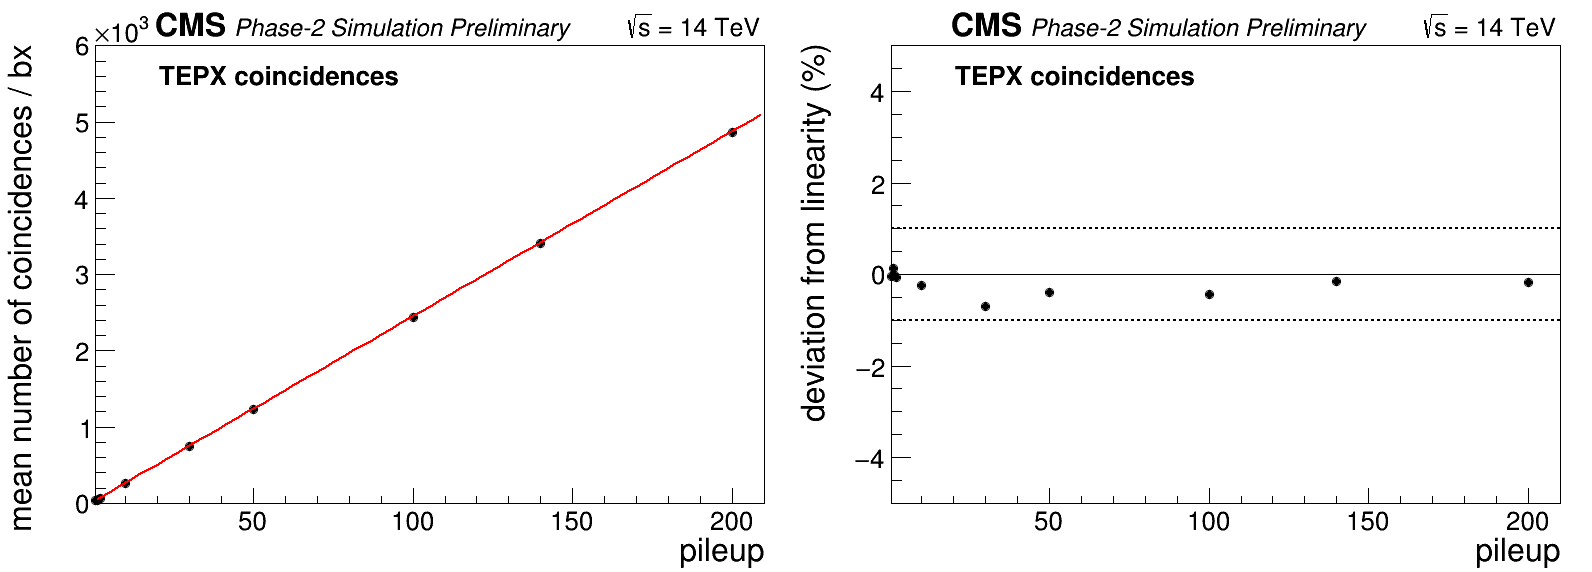
\includegraphics[width=1 \columnwidth]{./totalcoincidences.png}
  \caption{Left: Simulated mean number of coincidences in $\phi$ and r for all entire TEPX detector as a function of pileup. A line is fitted between pileup values of 0 and 2, and then extrapolated up to a pileup of 200. Right: Deviation from linearity for coincidence in $\phi$ and r for entire TEPX detector. The non-linearity is calculated as the relative difference between the data points and the values of the fit function at the respective pileup value. Non-linearity is within 1 \% for entire pileup range. Pileup 200 corresponds to High Luminosity (HL)-LHC environment.}
  \label{fig:CMS}
\end{figure}


\begin{figure}[H]
  \centering
  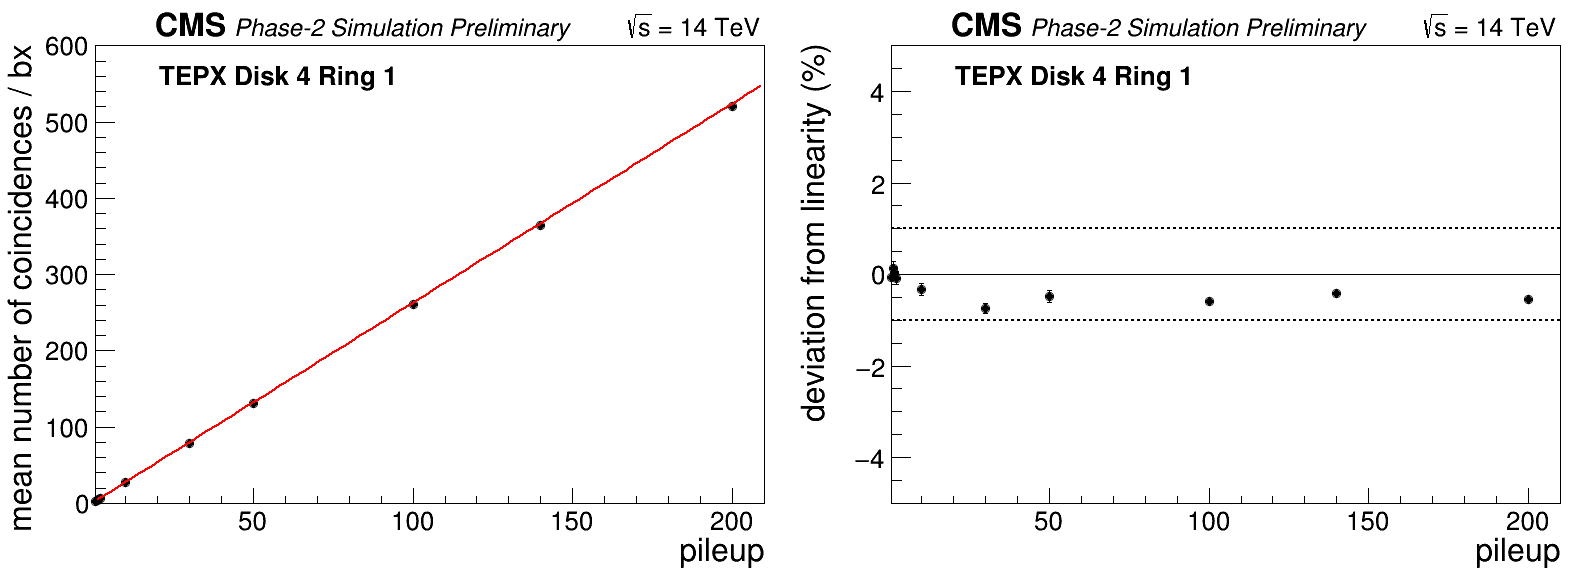
\includegraphics[width=1\columnwidth]{./totalcoincidencesD4R1.png}
  \caption{Left: Simulated mean number of coincidences in $\phi$ and r for TEPX Disk 4 Ring 1 as a function of pileup. Right: Deviation from linearity for coincidences in $\phi$ and r for TEPX Disk 4 Ring 1. The non-linearity is calculated as the relative difference between the data points and the values of the fit function at the respective pileup value.}
  \label{fig:CMS}
\end{figure}


\begin{figure}[H]
  \centering
  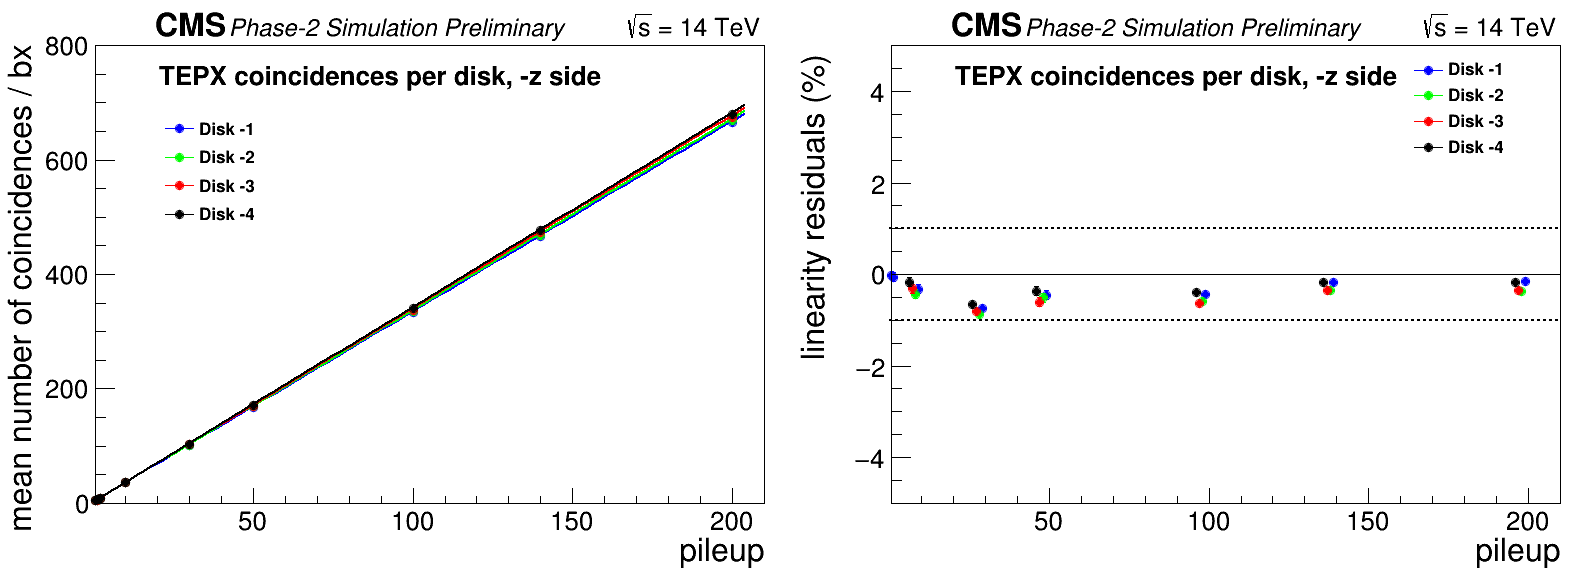
\includegraphics[width=1\columnwidth]{.//coincidencesperdisk-z.png}
  \caption{Left: Simulated mean number of coincidences in $\phi$ and r for -z side TEPX disks as a function of pileup. Right: Deviation from linearity for coincidences in $\phi$ and r for -z side TEPX disks.}
  \label{fig:CMS}
\end{figure}


\begin{figure}[H]
  \centering
  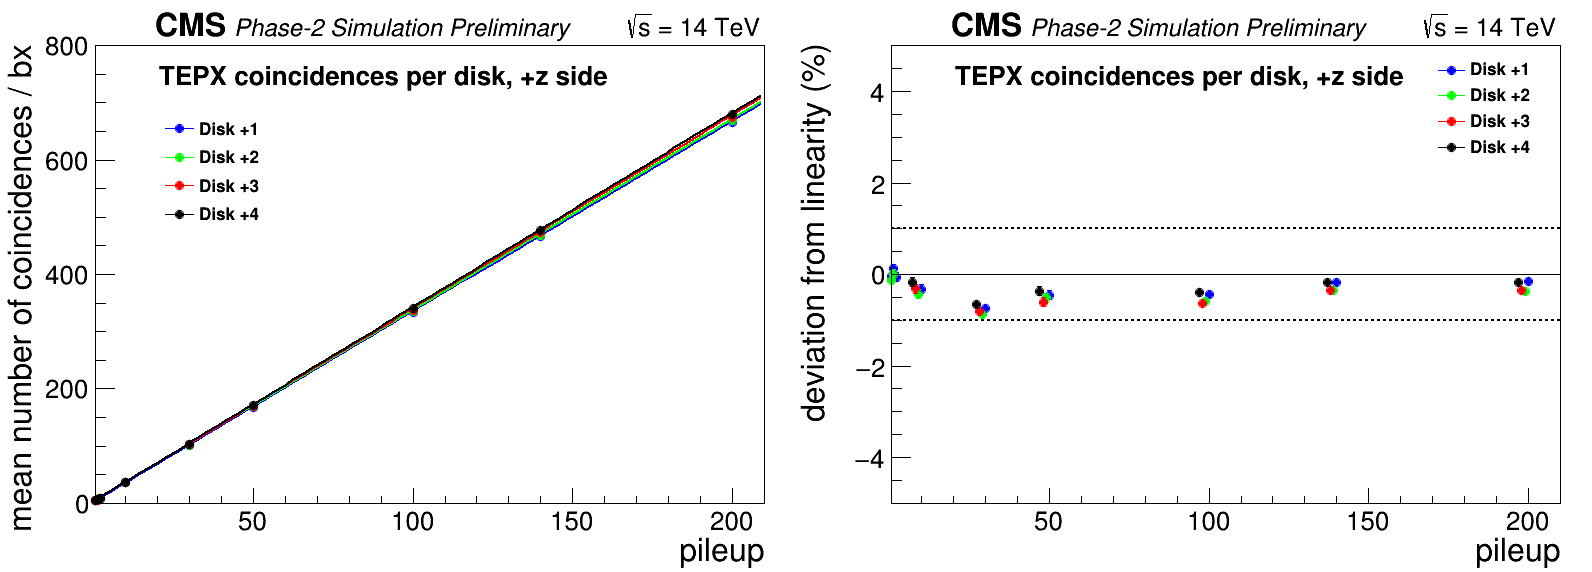
\includegraphics[width=1\columnwidth]{./coincidencesperdisk+z.png}
  \caption{Left: Simulated mean number of coincidences in $\phi$ and r for +z side TEPX disks as a function of pileup. Right: Deviation from linearity for coincidences in $\phi$ and r for +z side TEPX disks.}
  \label{fig:CMS}
\end{figure}







\begin{figure}[H]
  \centering
  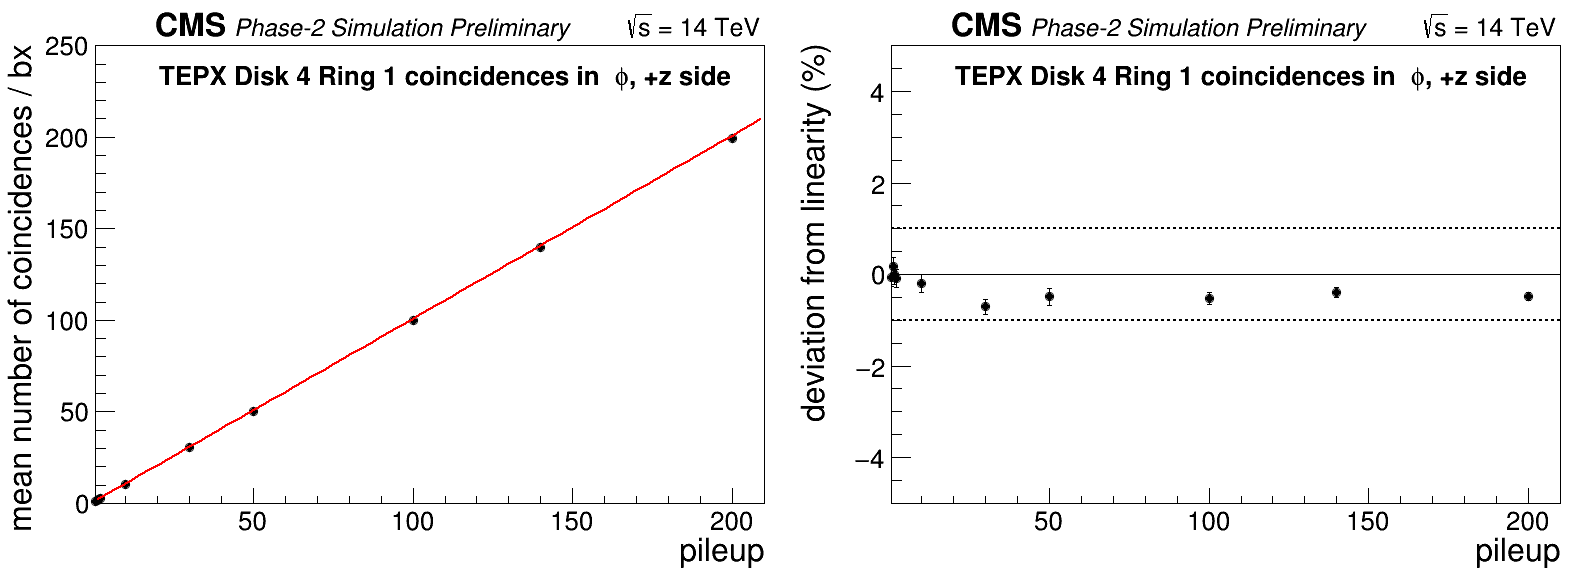
\includegraphics[width=1\columnwidth]{./coincidencesinphiD4R1z+.png}
  \caption{Left: Simulated mean number of coincidences in $\phi$ for TEPX +z side Disk 4 Ring 1 as a function of pileup. Right: Deviation from linearity for coincidences in $\phi$ for TEPX +z side Disk 4 Ring 1. The non-linearity is calculated as the relative difference between the data points and the values of the fit function at the respective pileup value.}
  \label{fig:CMS}
\end{figure}



\begin{figure}[H]
  \centering
  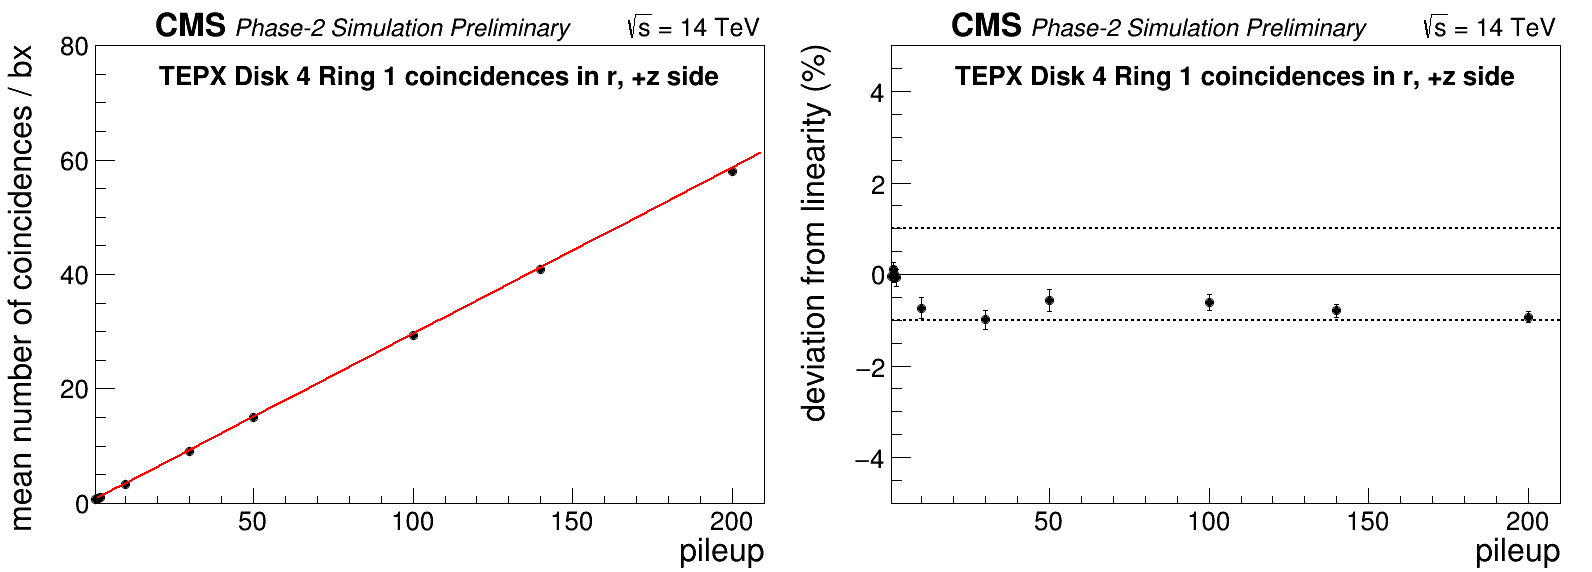
\includegraphics[width=1\columnwidth]{./coincidencesinrD4R1z+.png}
  \caption{Left: Simulated mean number of coincidences in r for TEPX +z side Disk 4 Ring 1 as a function of pileup. Right: Deviation from linearity for coincidences in r for TEPX +z side Disk 4 Ring 1. The non-linearity is calculated as the relative difference between the data points and the values of the fit function at the respective pileup value.}
  \label{fig:CMS}
\end{figure}


\begin{figure}[H]
  \centering
  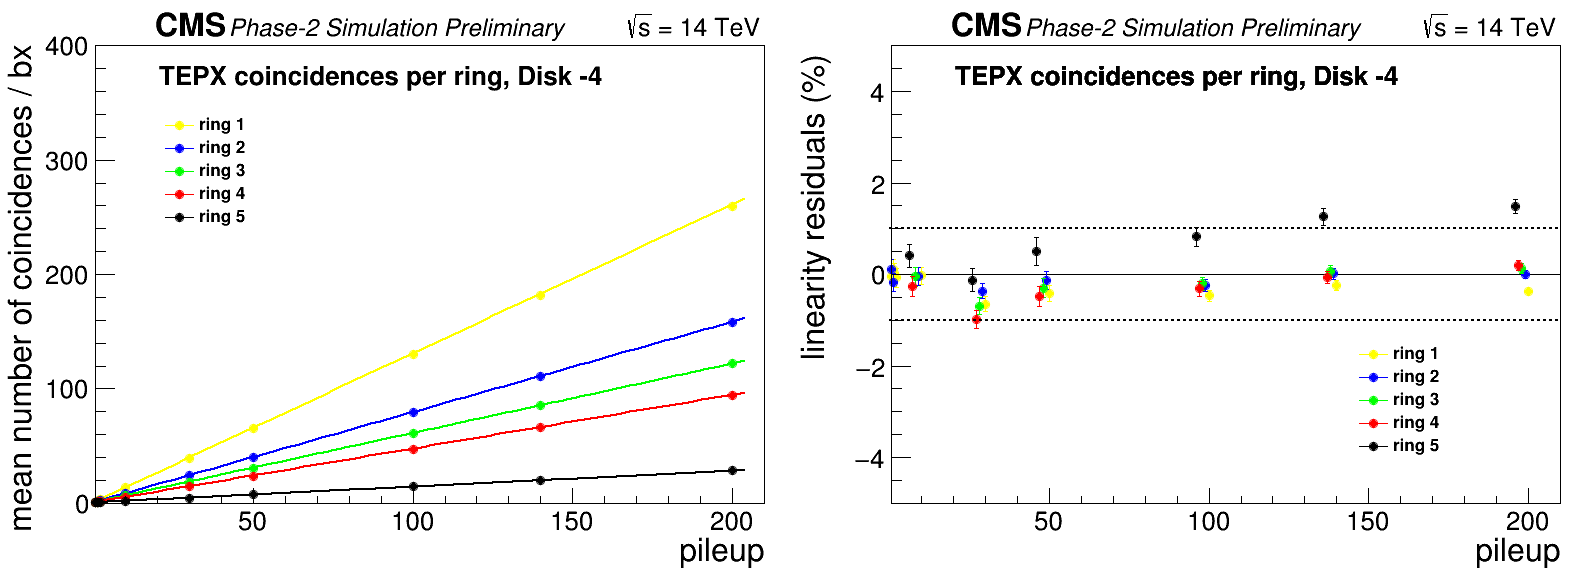
\includegraphics[width=1\columnwidth]{./coincidencesperringD-4.png}
  \caption{Left: Simulated mean number of coincidences in $\phi$ and r for -z side TEPX Disk 4 per ring as a function of pileup. Ring 1 has highest slope and Ring 5 has least slope. Right: Deviation from linearity for coincidences in $\phi$ and r for -z side TEPX Disk 4 per ring. Non-linearity is within 1\% for all rings over entire pileup range.}
  \label{fig:CMS}
\end{figure}


\begin{figure}[H]
  \centering
  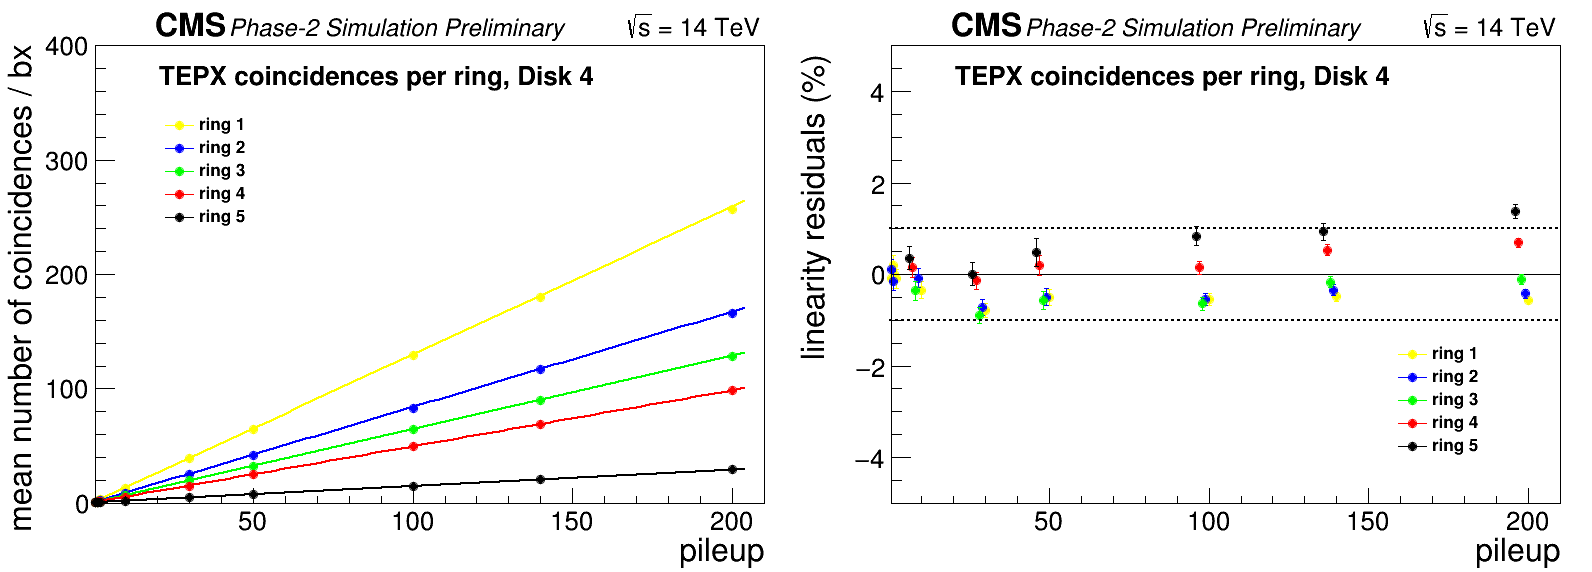
\includegraphics[width=1\columnwidth]{./coincidencesperringD+4.png}
  \caption{Left: Simulated mean number of coincidences in $\phi$ and r for +z side TEPX Disk 4 per ring as a function of pileup. Ring 1 has highest slope and Ring 5 has least slope. Right: Deviation from linearity for coincidences in $\phi$ and r for +z side TEPX Disk 4 per ring. Non-linearity is within 1\% for all rings over entire pileup range.}
  \label{fig:CMS}
\end{figure}






\begin{figure}[H]
  \centering
  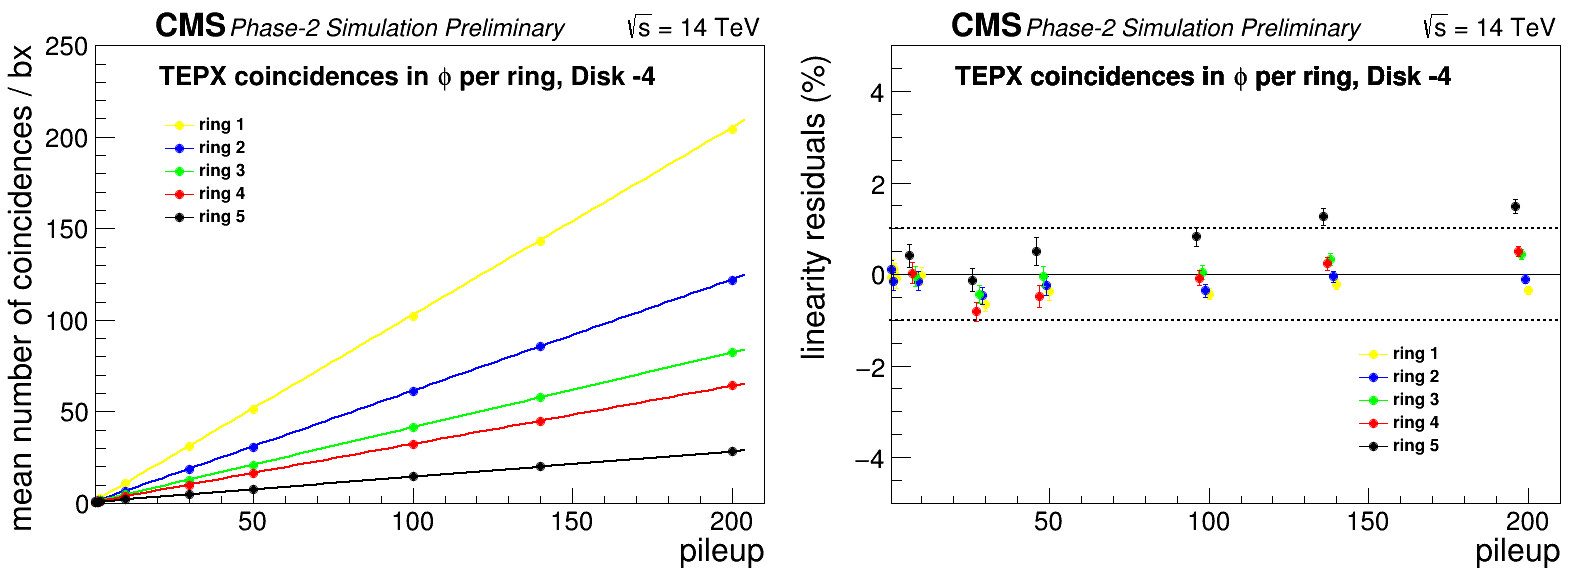
\includegraphics[width=1\columnwidth]{./coincidencesinphiperringD-4.png}
  \caption{Left: Simulated mean number of coincidences in $\phi$ for -z side TEPX Disk 4 per ring as a function of pileup. Ring 1 has highest slope and Ring 5 has least slope. Right: Deviation from linearity for coincidences in $\phi$ for -z side TEPX Disk 4 per ring. Non-linearity is within 1\% for all rings over entire pileup range.}
  \label{fig:CMS}
\end{figure}

\begin{figure}[H]
  \centering
  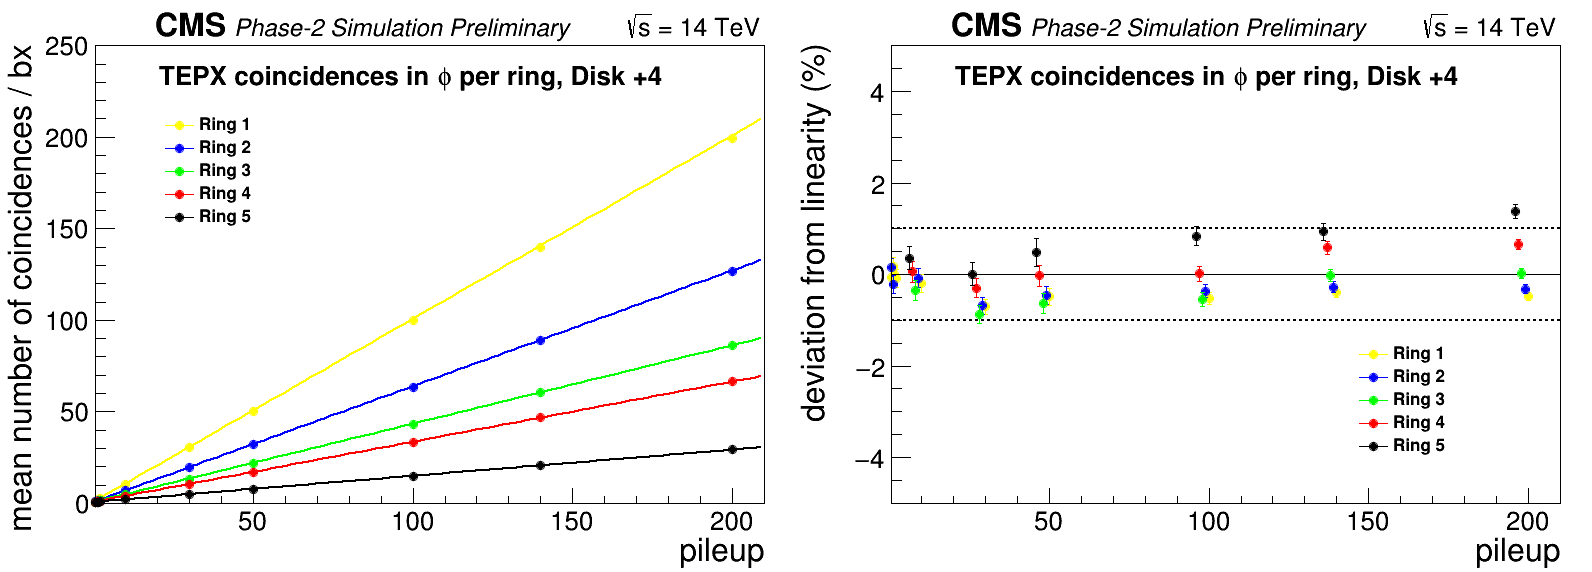
\includegraphics[width=1\columnwidth]{./coincidencesinphiperringD+4.png}
  \caption{Left: Simulated mean number of coincidences in $\phi$ for +z side TEPX Disk 4 per ring as a function of pileup. Ring 1 has highest slope and Ring 5 has least slope. Right: Deviation from linearity for coincidences in $\phi$ for +z side TEPX Disk 4 per ring. Non-linearity is within 1\% for all rings over entire pileup range.}
  \label{fig:CMS}
\end{figure}


\begin{figure}[H]
  \centering
  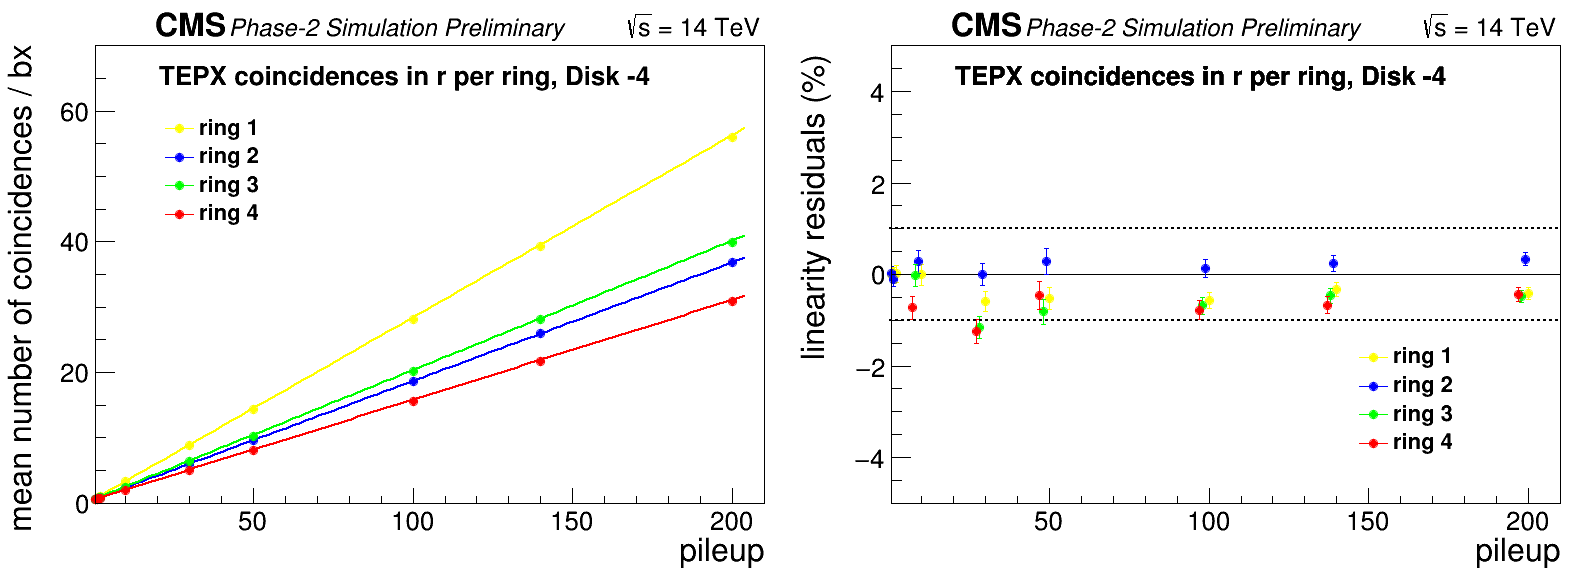
\includegraphics[width=1\columnwidth]{./coincidencesinrperringD-4.png}
  \caption{Left: Simulated mean number of coincidences in r for -z side TEPX Disk 4 per ring as a function of pileup. Ring 1 has highest slope and Ring 5 has least slope. Right: Deviation from linearity for coincidences in r for -z side TEPX Disk 4 per ring. Non-linearity is within $1\%$ for all rings over entire pileup range.}
  \label{fig:CMS}
\end{figure}


\begin{figure}[H]
  \centering
  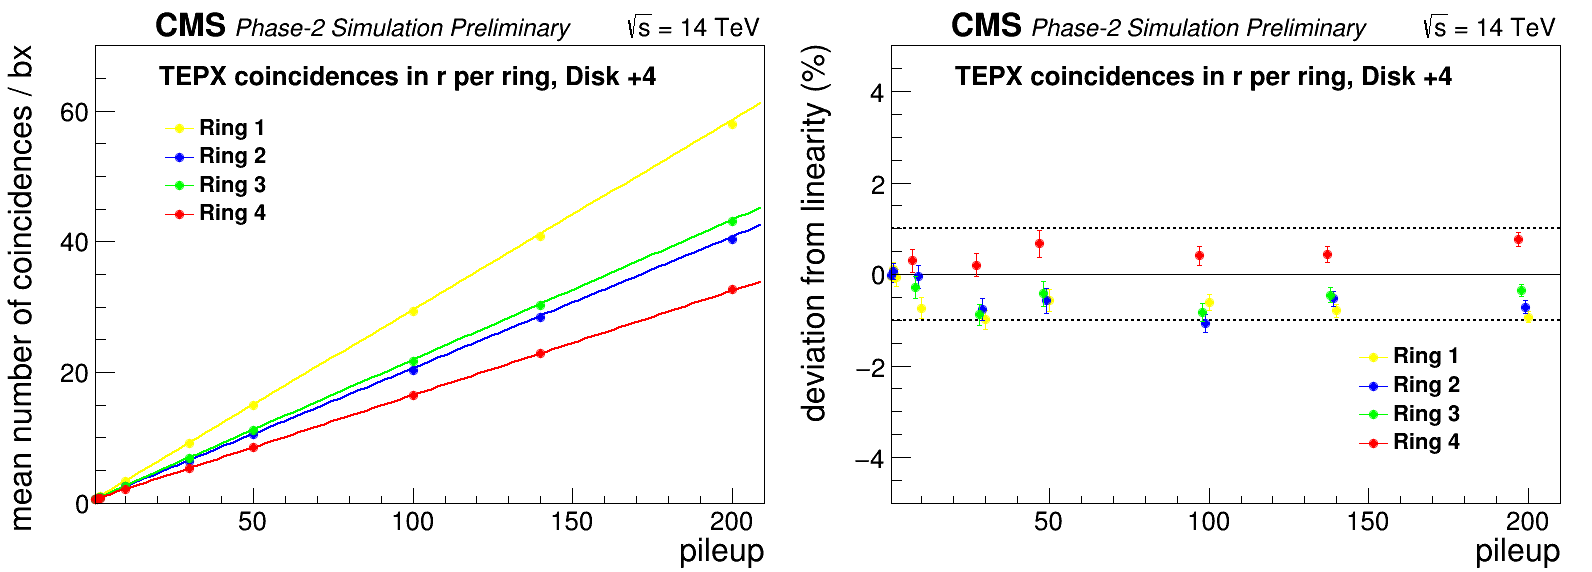
\includegraphics[width=1\columnwidth]{./coincidencesinrperringD+4.png}
  \caption{Left: Simulated mean number of coincidences in r for +z side TEPX Disk 4 per ring as a function of pileup. Ring 1 has highest slope and Ring 5 has least slope. Right: Deviation from linearity for coincidences in r for +z side TEPX Disk 4 per ring. Non-linearity is within $1\%$ for all rings over entire pileup range.}
  \label{fig:CMS}
\end{figure}







VdM (PU 0.5) $\:\:$  Trigger frequency (kHz) $\:\:$ 1 bx, 30 s $\:\:$ 100 bx, 30 s \\
TEPX D4R1 2x Coincidences in $\phi$  $\:\:$  800        $\:\:$   1.7         $\:\:$       0.17   \\
TEPX 2x Coincidences in $\phi$   $\:\:$     500        $\:\:$   0.485       $\:\:$       0.0485   \\




Physics (PU 200)  $\:\:$ Trigger frequency (kHz)   $\:\:$   1 bx, 4 LN (1.46 s)   $\:\:$     2500 bx, 1 LS (23 s)  \\
                                                      $\:\:$           ``Online''          $\:\:$           ``Offline''      \\
TEPX D4R1 2x Coincidences in $\phi$  $\:\:$   800                $\:\:$   0.386           $\:\:$            0.00193         \\
TEPX 2x Coincidences in $\phi$       $\:\:$   75           $\:\:$         0.284           $\:\:$            0.00142         \\



\chapter{Conclusiones}

En esta tesis se ha llevado a cabo un análisis exhaustivo del modelo de ruido para la medición de luminosidad utilizando el método de conteo de clusters de píxeles (PCC) en el experimento CMS. A través de este estudio, se ha demostrado que el método PCC es una herramienta robusta y precisa para medir la luminosidad, gracias a su alta granularidad y baja ocupación en el detector de píxeles de silicio. La observación y caracterización del afterglow, tanto de tipo 1 como de tipo 2, ha permitido comprender mejor los efectos residuales que influyen en las mediciones de luminosidad, lo que es crucial para garantizar la precisión de los datos obtenidos en el LHC.

El modelo matemático propuesto, que incluye contribuciones del afterglow y del ruido residual, ha mostrado un buen ajuste a los datos experimentales, como lo evidencian los residuos distribuidos aleatoriamente alrededor de cero. Además, el análisis de la evolución temporal de los parámetros del modelo ha revelado que estos presentan un comportamiento estable a lo largo del tiempo, lo que refuerza la validez del modelo utilizado.

En resumen, este trabajo contribuye a mejorar la precisión de las mediciones de luminosidad en el experimento CMS, lo que es fundamental para la búsqueda de nuevas partículas, la medición de las propiedades de partículas conocidas y la detección de procesos raros. Los resultados obtenidos abren nuevas perspectivas para futuros estudios en física de partículas, especialmente en lo que respecta a la optimización de los métodos de medición de luminosidad en colisionadores de alta energía.



\cleardoublepage
\onehalfspacing
\bibliographystyle{unsrt}
\bibliography{paper}

\end{document}




